%%%%%%%%%%%%%%%%%%%%%%%%%%%%%%%%%%%%%%%%%%%%%%%%%%%%%%%%%%%%%%%%%%%%%%%%%%
%%        file: atprog-thesis-template-eng-20190426.tex
%%      author: Heiki Kasemgi <heiki.kasemagi@eesti.ee>
%% description: tex source
%% computer engineering
%% thesis template
%% copyright (c) 2015-2019, Heiki Kasemägi, <heiki.kasemagi@eesti.ee>
%%
%% 297x210 format A4
%%
%% double "%" marks a comment
%% single "%" marks a commented command
%% the complete set of (commented) commands is between the lines marked as 
%% "%%=== title ===" and "%%%%%%%%%"
%%%%%%%%%%%%%%%%%%%%%%%%%%%%%%%%%%%%%%%%%%%%%%%%%%%%%%%%%%%%%%%%%%%%%
%% This program is free software; you can redistribute it and/or
%% modify it under the terms of the GNU General Public License
%% as published by the Free Software Foundation; either version 2
%% of the License, or (at your option) any later version.
%%
%% This program is distributed in the hope that it will be useful,
%% but WITHOUT ANY WARRANTY; without even the implied warranty of
%% MERCHANTABILITY or FITNESS FOR A PARTICULAR PURPOSE.  See the
%% GNU General Public License for more details.
%%
%% You should have received a copy of the GNU General Public License
%% along with this program; if not, write to the Free Software
%% Foundation, Inc., 51 Franklin Street, Fifth Floor, Boston,
%% MA  02110-1301, USA
%%
%%%%%%%%%%%%%%%%%%%%%%%%%%%%%%%%%%%%%%%%%%%%%%%%%%%%%%%%%%%%%%%%%%%%%%%%%%
%% Käesolev programm on vaba tarkvara. Te võte seda edasi levitada ja/või
%% muuta vastavalt GNU Üldise Avaliku Litsentsi tingimustele, nagu need on
%% Vaba Tarkvara Fondi poolt avaldatud; kas Litsentsi versioon number 2
%% või (vastavalt Teie valikule) ükskõik milline hilisem versioon.
%%
%% Seda programmi levitatakse lootuses, et see on kasulik, kuid ILMA
%% IGASUGUSE GARANTIITA; isegi KESKMISE/TAVALISE KVALITEEDI GARANTIITA või
%% SOBIVUSELE TEATUD KINDLAKS EESMRGIKS. Üksikasjade suhtes vaata GNU
%% Üldist Avalikku Litsentsi
%%
%% Te peaks olema saanud GNU Üldise Avaliku Litsentsi koopia koos selle
%% programmiga, kui ei, siis kontakteeruge Free Software Foundation'iga,
%% 59 Temple Place - Suite 330, Boston, MA 02111-1307, USA
%%
%%%%%%%%%%%%%%%%%%%%%%%%%%%%%%%%%%%%%%%%%%%%%%%%%%%%%%%%%%%%%%%%%%%%%%%%%%

\documentclass[12pt]{report}
\usepackage{a4}
\usepackage{amsmath}
\usepackage{xcolor}
%\usepackage{fancyhdr}
\usepackage[nottoc]{tocbibind} % option removes the "Contents" form the
% contents
\usepackage{times}
\usepackage{cite}
\usepackage{graphicx}
\usepackage{rotating}
\usepackage{hyperref}
\usepackage[nopar]{lipsum} % package for dummmy texts
\usepackage{titlesec}
\usepackage{enumitem}
\usepackage{adjustbox}
\usepackage{listings}

%% For JavaScript 

\usepackage{listings}
\usepackage{color}
\definecolor{lightgray}{rgb}{0.95,0.95,0.95}
\definecolor{darkgray}{rgb}{.4,.4,.4}
\definecolor{purple}{rgb}{0.65, 0.12, 0.82}

\lstdefinelanguage{JavaScript}{
  keywords={typeof, new, true, false, catch, function, return, null, catch, switch, var, if, in, while, do, else, case, break},
  keywordstyle=\color{blue}\bfseries,
  ndkeywords={class, export, boolean, throw, implements, import, this},
  ndkeywordstyle=\color{darkgray}\bfseries,
  identifierstyle=\color{black},
  sensitive=false,
  comment=[l]{//},
  morecomment=[s]{/*}{*/},
  commentstyle=\color{purple}\ttfamily,
  stringstyle=\color{red}\ttfamily,
  morestring=[b]',
  morestring=[b]"
}

\lstset{
   language=JavaScript,
   backgroundcolor=\color{lightgray},
   extendedchars=true,
   basicstyle=\footnotesize\ttfamily,
   showstringspaces=false,
   showspaces=false,
   numbers=left,
   numberstyle=\footnotesize,
   numbersep=9pt,
   tabsize=2,
   breaklines=true,
   showtabs=false,
   captionpos=b
}

%\usepackage{ccaption}
%%=== B5 page setup ===
%\setlength{\paperwidth}{17.5cm} %B5
%\setlength{\paperheight}{25cm} %B5
%\setlength{\textwidth}{12.5cm} %B5
%\setlength{\textheight}{19.5cm} %B5
%%%%%%%%%%%%%%%%%%%%%%%%%%%%%%%%%%%%
%%=== A4 page setup ===
\setlength{\paperwidth}{21.0cm} 
\setlength{\paperheight}{29.7cm}
\setlength{\textwidth}{16cm}
\setlength{\textheight}{25cm}
%%%%%%%%%%%%%%%%%%%%%%%%%%%%%%%%%%%
%%=== common ===
\setlength{\leftmargin}{2.5cm} %2.5cm
\setlength{\rightmargin}{2.5cm} %2.5cm
\setlength{\oddsidemargin}{0cm}
\setlength{\evensidemargin}{0cm}
\setlength{\topmargin}{-2.0cm} %-2.0cm
%%\setlength{\headsep}{0.0cm}
%%\setlength{\headheight}{0.0cm}
\setlength{\footskip}{1.0cm} %-2.5cm
\setlength{\topskip}{0.5cm}
%%%%%%%%%%%%%%%%%%%%%%%%%%%%%%%%%%%%%%
%%=== watermark setup ===
%\usepackage[outline,light,portrait]{draftcopy}
%\draftcopyName{Heiki Kasemagi Ph. D. Thesis}{45}
%\draftcopyPageX{30}
%\draftcopyPageY{50}
%\draftcopyBottomX{0}
%\draftcopyBottomY{-100}
%%%%%%%%%%%%%%%%%%%%%%%%%%%%
%\renewcommand{\thefigure}{\arabic{figure}}
%\renewcommand{\figurename}{Figure}
%\setcounter{figure}{0}
%%=== 1.5 row spacing ===
%\renewcommand{\baselinestretch}{1.5}
%%%%%%%%%%%%%%%%%%%%%%%%%%%%%%
%%=== disabling the hypenation ===
%\hyphenpenalty=1000
%%%%%%%%%%%%%%%%%%%%%%%%%%%%%%
%%\renewcommand{\contentsname}{\protect \center{Contents}}
%%\renewcommand{\listfigurename}{\protect \centering List of Figures}
%%\renewcommand{\chaptername}{\protect \centering Chapter}
%%=== translations to Estonian ===
%%=== comment for English ===
%%%\renewcommand{\bibname}{References}
%%%\renewcommand{\contentsname}{Content}
%%%\renewcommand{\listfigurename}{Jooniste loetelu}
%%%\renewcommand{\listtablename}{Tablelite loetelu}
%\renewcommand{\chaptername}{}
%%%\renewcommand{\figurename}{Joonis}
%%%\renewcommand{\tablename}{Tabel}
%%%%%%%%%%%%%%%%%%%%%%%%%%%%%%%%
%%=== ===
%%\makeatletter
%%\renewcommand{\section}{\@startsection{section}{1}{0mm}
%%{\baselineskip}%
%%{\baselineskip}{\Large\centering}}%
%%\makeatother
%%%%%%%%%%%%%%%%%%%%%%%%%%%%%%%%

%%%========== make own fig caption not listed in LOF ==========
\newcommand\myCaption[1]{\normalsize\refstepcounter{figure}%
   \figurename\ \thefigure :\ #1}
%%%============================================================

%%%========== remove page number for TOC ==========
%\makeatletter
%\let\myTOC\tableofcontents
%\renewcommand{\tableofcontents}{%
%  \begingroup
%  \let\ps@plain\ps@empty
%  \pagestyle{empty}
%  \myTOC
%%  \clearpage
%  \endgroup%
%}
%\makeatother
%%%================================================
%%=== insert figure ===
%% arguments: 
%% #1 - figure location in the page, recommended "h"
%% #2 - figure width, recommended "x.x\textwidth" where x.x is a fraction
%%      of the page width, e.g. "0.54\textwidth" is 54 % of the text width
%% #3 - figure path
%% #4 - figure caption
%% #5 - figure label for referencing in the text
\newcommand\insertfigure[5]{
\begin{figure}[#1]
\begin{center}
\includegraphics[width=#2]{#3}
\end{center}
\caption{#4}
\label{#5}
\end{figure}
}
%%%%%%%%%%%%%%%%%%%%%%%%%%%%%%%%%%%%%%%%%%%
%%=== modified chapter title ===
\newcommand{\hsp}{\hspace{20pt}}
\titleformat{\chapter}[hang]{\Huge\bfseries}{\thechapter\hsp}{0pt}{\Huge\bfseries}
%%%%%%%%%%%%%%%%%%%%%%%%%%%%%%%%%%%%%%%%%%%

\begin{document}
%\noindent
\thispagestyle{empty}
%%=== titlepage ===
\begin{large}
\begin{center}
\vspace{20mm}
Tartu University
\\[5mm]
Faculty of Science and Technology
\\[5mm]
Institute of Technology
\\[5mm]
\vspace{50mm}
Lilou Gras
\\[10mm]
\textbf{Exploring Reinforcement Learning for Autonomous Control: A Case Study with the OpenBot Platform}
\\[10mm]
Master's thesis (30 EAP)\\
Robotics and Computer Engineering\\
%Magistrit\"o\"o (30 EAP)\\
\end{center}
\vspace{20mm}
\flushright{Supervisor: Dr. Naveed Muhammad}
%\flushright{Juhendajad:}
\\[5mm]

%amet Eesnimi Perekonnanimi\\
%%...
\begin{center}
%% adjust vspace value according to title rows and supervisor count
\vspace{65mm}
Tartu 2023\\
\end{center}
\end{large}
\newpage
%%=== Abstract ===
\chapter*{Abstract}
\addcontentsline{toc}{chapter}{Abstract}
\textbf{Exploring Reinforcement Learning for Autonomous Control: A Case Study with the OpenBot Platform}
\\[5mm]
This thesis investigates the application of reinforcement learning (RL) in the context of the OpenBot platform, emphasizing its comparative effectiveness with traditional machine learning for data gathering and circuit navigation, particularly in a lane following scenario. The primary objective is to implement RL within the OpenBot app and Python scripts for semi-online reinforcement learning, deviating from the conventional practice of training in simulated environments by conducting experiments on real hardware.

The methodology involves training the OpenBot to follow a lane and complete laps of a circuit using a reward function integrated into the loss to be maximized. The results indicate that both RL and traditional machine learning methods achieved the desired outcomes, yet RL required significantly more assistance and time—approximately 8 to 10 hours, compared to the approximately 2 hours needed for traditional machine learning.

The comparative analysis highlights the strengths and challenges associated with RL and traditional machine learning methodologies. Notably, the superior lane-following performance demonstrated by RL is attributed to meticulous data curation and the incorporation of a substantial punishment for deviations from the lane. However, considerations of time efficiency, autonomy, and intuitiveness reveal the superiority of machine learning in these domains.

For future work, avenues include building a new RL model from scratch, refining the reward function, exploring different tasks with new reward functions, improving the automation of the process to reduce time consumption, and adapting scripts for compatibility with various platforms capable of sending data to Python servers.

In conclusion, this research not only contributes valuable insights into the practical implementation of RL in mobile robotics but also underscores the importance of considering diverse methodologies to meet specific challenges. 
\\[5mm]
\textbf{CERCS:} : T125 Automation, robotics, control engineering;  P170 Computer science, numerical analysis, systems, control
\\[5mm]
\textbf{Keywords:} Semi-Online Reinforcement Learning, Control, Robotics, Autonomous Driving, OpenBot Platform, Real Hardware Experiments

\newpage
\noindent \textbf{Autonoomse juhtimise jaoks poolvõrgupõhise tugevdamise õppimise uurimine: juhtumiuuring OpenBoti platvormiga}
\\[5mm]

\noindent See lõputöö uurib täiendusõppe (RL) (ingl: reinforcement learning) rakendamist OpenBoti platvormi kontekstis, rõhutades selle efektiivsust traditsioonilise masinõppega võrreldes andmete kogumisel ja ringirajade navigeerimisel, eriti stsenaariumi järgimisel. Põhiline eesmärk on RL-i juurutamine OpenBoti rakenduses ja Pythoni skriptides pooleldi võrgupõhiseks täiendusõppeks, tehes katseid reaalse riistvaraga selle asemel, et treenida tavapärastes simuleeritud keskkondades.

Metoodika hõlmab OpenBoti koolitamist, et ta järgiks rada ja läbiks ringrada, kasutades maksimeerimiseks integreeritud preemiafunktsiooni. Tulemused näitavad, et nii RL kui ka traditsioonilised masinõppemeetodid saavutasid soovitud järelmi, kuid RL vajas masinõppest oluliselt rohkem toetust ja aega – ligikaudu 8–10 tundi, võrreldes traditsioonilisele masinõppele
kuluva umbes 2 tunniga.

Võrdlev analüüs toob esile RL-i ja traditsiooniliste masinõppe metoodikatete tugevad ja väljakutseid pakkuvad küljed. Tähelepanuväärselt on RL-i parem raja jälgimine tingitud andmete täpsest haldamisest ja rajalt kõrvalekaldumise eest tugeva karistuse kaasamisest. Siiski näitab aja tõhususe, autonoomia ja intuitsiooni kaalutluste valdkondades oma paremust masinõpe.

Edaspidiseks tööks on võimalik uue RL-mudeli algusest ehitamine, tasustamise funktsiooni täiustamine, protsessi automatiseerimise edendamine ajakulu vähendamiseks ja skriptide kohandamine erinevate platvormidega, mis on võimelised Pythoni serveritesse andmeid saatma. \footnotemark{}
\\[5mm]
\textbf{CERCS:} : T125 - Automatiseerimine, robootika, control engineering; P170 - Arvutiteadus, arvutusmeetodid, süsteemid, juhtimine  
\\[5mm]
\textbf{Keywords:} Täiendusõpe (reinforcement learning), OpenBoti platvorm, Võrgupõhine täiendusõpe, Riistvara, robootika, control

\footnotetext{This abstract was translated by Helena Plans from Fiverr \cite{bib:fiverr}}
%%=== let's add the table of contents, list of figures and tables ===
\tableofcontents
\listoffigures

%%=== list of abbreviations, constants etc. ===
\chapter*{Abbreviations, Constants, Generic Terms}
\addcontentsline{toc}{chapter}{Abbreviations. Constants. Generic Terms}
\begin{description}
\item[RL] - Reinforcement Learning
\item[DRL] - Deep Reinforcement Learning 
\item[DQN] - Deep Q Network
\item[NFQ] - Neural Fitted Q Iteration
\item[OTG] - On-The-Go
\item[RTR] - Ready-To-Run
\item[DRL] - Deep Reinforcement Learning 
\item[MSE] - Mean Squared Error
\item[MoR] - Mean of Rewards


\end{description}
%%=== chapter: introduction ===
\chapter{Introduction}
\label{sub:Introduction}

The use of reinforcement learning in robotics is becoming increasingly important, especially in mobile robotics. This change not only offers more independence to robots but also enables them to learn and adjust in real-world situations. Mobile robotics, which naturally requires adaptability, aligns well with reinforcement learning, opening up possibilities for smart navigation. At the same time, smartphones, widely used for their strong computing abilities and effective sensors, are a great tool for connecting theoretical algorithms to practical uses in robotics. Besides their technical abilities, smartphones are very accessible. This study sets out on a unique journey, aiming to introduce reinforcement learning into mobile robotics through the familiar interface of a smartphone using the OpenBot platform \cite{bib:openbot}. By using the accessibility of this platform, the goal is to make the integration of advanced learning algorithms more approachable for educational purposes. This combination of reinforcement learning, mobile robotics, and smartphones represents a promising area.

%%=== section: problem overview ===
\section{Problem Statement}
\label{sub:Problem_Statement}

Integration of reinforcement learning appears promising in the realm of mobile robotics, yet its application can be challenging. Currently, most research tend to rely on simulated environments or high-performance computational setups. There is less research done regarding real-world implementation of reinforcement learning algorithms. This research gap is even more pronounced in the context of robots controlled by smartphones, which have limited computational power, and in which deep learning libraries are still in the experimental phase. 


This study aims to fill this gap by exploring the challenges linked to applying reinforcement learning algorithms in real-world situations, concentrating specifically on a robot controlled by smartphones. By tackling the difficulties arising from limited computational resources, this research strives to provide insights and solutions for the incorporation of reinforcement learning using the accessible OpenBot platform.

%%=== section: goals ===
\section{Roadmap and Objectives}
\label{sub:Roadmap and Objectives}

In this section, we provide an overview of the roadmap that will guide our exploration and the objectives we aim to achieve throughout this research.


\subsection{Roadmap}
This document is structured into six chapters, each addressing specific aspects of the research:

\paragraph{Chapter 1: Introduction}
In this chapter \ref{sub:Introduction}, the identified problem is discussed in the Problem Statement section. The Roadmap and Objectives section outlines the structure of the document and the goals of the research.

\paragraph{Chapter 2: State of the Art}
This chapter \ref{sub:State_of_the_art} explores the OpenBot platform, describing its hardware components \ref{sub:Hardware_Components}, assembly \ref{sub:Mechanical_assembly}, software integration \ref{sub:Software_integration}. Then Reinforcement Learning concepts \ref{sub:Rapid_intro_RL} and their origins are introduced \ref{sub:Beginning_RL}. Additionally, it examines the current trends in reinforcement learning with real robotics implementation \ref{sub:SOTA_trends_RL} and highlights the specific contributions of the present study \ref{sub:Contribution_present_study}.

\paragraph{Chapter 3: Methodology}

In this chapter \ref{sub:Methodology}, the methodology unfolds, starting with the development of the Android app for control \ref{sub:Android_app} within the OpenBot repository. The process involves gaining a thorough understanding of the OpenBot repository and app \ref{sub:Understanding_openbot}, integrating the OpenCV library \ref{sub:Integration_of_OpenCV_Library}, implementing new features \ref{sub:Implementation_of_New_Features}, and conducting careful testing and debugging \ref{sub:Testing_and_debugging}. Following this, the rationale behind our experimental design is explained, covering the lane following scenario \ref{sub:lane}, computational constraints \ref{sub:Computational_constraints} requiring semi-online learning, and the thoughtful selection of model and loss function \ref{sub:Choice_of_model}. The experiment design is detailed, including the circuit \ref{sub:circuit}, procedural steps \ref{sub:step}, and security measures \ref{sub:security}. The subsequent sections explore implementation aspects, including the design of the reward function \ref{sub:Designing_the_reward_function}, modification of the OpenBot app \ref{sub:Modification_of_openbot}, presentation of Python scripts \ref{sub:python}, data preprocessing \ref{sub:preprocessing}, addition of rewards to the dataloader and TensorFlow records \ref{sub:reward}, modification of the train.py script \ref{sub:mod_train}, and the description of a Python server for data transmission \ref{sub:server}.

\paragraph{Chapter 4: Results}
The results obtained through the application of reinforcement learning \ref{sub:results_rl} and traditional machine learning \ref{sub:results_ml} are presented and discussed in this chapter \ref{sub:Results}.

\paragraph{Chapter 5: Analysis and Discussion}
This chapter \ref{sub:Analysis_and_discussion} analyzes the results obtained through reinforcement learning \ref{sub:analysis_rl} with OpenBot and traditional machine learning \ref{sub:analysis_ml}. It includes a comparison of the results \ref{sub:compare} and outlines future steps for further research \ref{sub:future}.

\paragraph{Chapter 6: Conclusion}
The final chapter \ref{sub:Conclusion} summarizes the key findings, discusses future perspectives for research in this domain, and concludes the document.

\subsection{Objectives}


\subsubsection{Primary Objective:}

Implement Reinforcement Learning (RL) in the OpenBot platform and compare its performance with traditional machine learning for data gathering and circuit navigation in a lane following scenario. Specifically, the primary goal is to assess the efficiency and success of RL training on real hardware, deviating from the typical simulation-based approach.

\subsubsection{Secondary Objective:}

Explore the potential of integrating RL into educational platforms as a means of facilitating learning and understanding of RL concepts. This involves assessing the feasibility and effectiveness of using OpenBot as an educational tool to teach RL principles. The secondary objective aims to contribute insights into the educational applications of RL in a practical and accessible manner.

%%=== chapter: problem review ===
\chapter{State of the Art}
\label{sub:State_of_the_art}
This section introduces OpenBot as an accessible and innovative platform for real-world experimentation and provides an introduction to Reinforcement Learning (RL) principles and first works. 


As the current state of RL in real mobile robotics is examined, challenges such as computational intensity and training mostly done in simulated environments are brought to light. Both advancements and persistent challenges in RL applications are illustrated by various studies, spanning from walking robots \cite{bib:walk} to real car driving \cite{bib:realcar}. 


The section wraps up by pointing out what makes this study unique and persistent. By concentrating on hardware robotics using OpenBot, this research uses semi-online RL to tackle computing challenges, offering practical insights.

\section{OpenBot, an accessible and innovative platform}
\label{sub:Openbot_accessible}
In this section, the detailed setup of the robotic car is presented, with the OpenBot platform \cite{bib:openbot} serving as the foundation for the experimental framework. The OpenBot platform is known as an accessible system that enables the conversion of a smartphone into a functional robotic platform. By leveraging the computational capabilities of the smartphone and its integrated sensors, a cost-effective solution is provided by the OpenBot platform for creating and exploring a wide range of robotic applications.

\subsection{Hardware Components}
\label{sub:Hardware_Components}

The OpenBot platform utilizes the following key hardware components:
\begin{itemize}
    \item A standard RC car chassis, either bought or 3D printed. 
    \item Four DC motors with tires for propulsion.
    \item An Android smartphone, serving as the primary computing unit, integrated with the OpenBot app. In this experimental framework, a Redmi Note 11 \cite{bib:phone} was used.
    \item Arduino Nano
    \item Custom PCBs
    \item A USB on-the-go (OTG) cable for communication between the smartphone and the microcontroller.
    \item Various sensors, including the smartphone's buit-in camera for vision-based navigation and, if applicable, additional sensors such as accelerometer, ultrasonic or push buttons for obstacle detection.
    \item Another phone or controller (PS4, Xbox,...) is required to send controls to the OpenBot.
\end{itemize}

For more information on how to build your robot, where to order it or about the custom PCBs, please refer to the OpenBot paper \cite{bib:openbot} and GitHub repository \cite{bib:git_openbot} listed in the bibliography. For this thesis, the OpenBot was the Ready-To-Run (RTR) model. 


\subsection{Mechanical Assembly \& Electrical Configuration}
\label{sub:Mechanical_assembly}



The OpenBot, depicted in Figure \ref{fig:RTR_TT}, is designed to be compact, housing its microcontroller, motors, and PCBs within the 3D printed mount. It features an adjustable smartphone mount suitable for various sizes. While the RTR model is chargeable, the DIY version operates using three 18650 batteries.


\insertfigure{th}{0.35\textwidth}{RTR_TT.jpg}{Picture of OpenBot with smartphone mounted. From OpenBot GitHub \cite{bib:git_openbot}.}{fig:RTR_TT}

\insertfigure{th}{0.7\textwidth}{wiring_diagram.png}{Wiring diagram. Electrical connections between battery, motor driver, microcontroller, speed sensors, sonar sensor and indicator LEDs. From the OpenBot GitHub and paper \cite{bib:openbot}\cite{bib:git_openbot}.}{fig:wiring_diagram}

Figure \ref{fig:wiring_diagram} illustrates the configuration with four motors and various components enclosed within the mount. The paired motors ensure synchronous control of the right and left wheels. In the event of a motor failure, the paired motor also ceases to operate despite receiving the command.




\subsection{Software Integration}
\label{sub:Software_integration}

The OpenBot platform was integrated with the smartphone's hardware and sensors through the OpenBot app, facilitating the communication and data exchange between the smartphone and the microcontroller.


The app offers various features, with the following being the most pertinent for this experiment:
\begin{itemize}
    \item \textbf{Autopilot}: This feature utilizes a customized tflite model uploaded to the smartphone, leveraging data from the phone and microcontroller as inputs. In a prior project \cite{bib:openbotLeonLilou}, this feature was successfully employed for autonomous navigation around a predefined circuit.
    \item \textbf{Model Management}: This feature provides a comprehensive interface for managing all uploaded models on the smartphone. Users can conveniently organize, delete, or download models, categorizing them as needed.
    \item \textbf{Data Collection}: A critical aspect of this experiment, the Data Collection feature records data from various sensors and the control log, saving the information in \texttt{.txt} or \texttt{.png} formats. This data is then uploaded to a remote Python server for machine learning algorithm training.
    \item \textbf{Free Roam}: This feature enables users to control the robot either through a controller or another Android phone equipped with the controller app, available on the OpenBot GitHub repository \cite{bib:git_openbot}.
\end{itemize}

\newpage
\section{Reinforcement Learning}
\subsection{Rapid Introduction to Reinforcement Learning}
\label{sub:Rapid_intro_RL}
\insertfigure{th}{0.55\textwidth}{RLOpenbot.png}{Illustration of the Reinforcement Learning Process: Agent-Environment Interaction and Reward System in the line following scenario.}{fig:RLOpenbot}

Reinforcement learning (RL) constitutes an important branch of machine learning that focuses on agents making decisions in dynamic environments. Unlike traditional supervised learning, where labeled datasets drive the learning process, RL relies on the concept of learning by interaction.




RL involves an agent, an environment, a state, actions, rewards, and a learning policy. The agent (OpenBot) is in a specific state (information from sensors such as images), takes actions (send commands to motors) in the environment (circuit), receiving rewards or penalties in response as seen in Figure \ref{fig:RLOpenbot}, which shapes its future decision-making through the learning policy as seen in Figure \ref{fig:learningPolicy}. This feedback loop forms the basis of the agent's learning process, where it strives to maximize cumulative rewards over time.
\insertfigure{th}{0.4\textwidth}{learningPolicy.png}{Simple Diagram of Reinforcement Learning Process, with live updates of the learning policy having direct impact on decision making, showed with the green dotted line.}{fig:learningPolicy}



\subsection{The beginning of Reinforcement Learning and pioneering works}
\label{sub:Beginning_RL}

Reinforcement learning has significantly evolved and showed noteworthy achievements since its beginnings. In the 1950s, foundational work was laid by Richard Bellman through dynamic programming \cite{bib:richard}, a methodology rooted in optimizing complex systems. Then in the 1980s, Q-learning was introduced by Christopher Watkins \cite{bib:delayed}, finding applications in adaptive control scenarios where optimal decision-making strategies are learned by agents.


A pivotal moment occurred in 1995 with the work of Gerald Tesauro on temporal difference learning \cite{bib:Tesauro}, demonstrating the efficacy of learning from experiences over time. 


The breakthrough of Deep Reinforcement Learning (DRL) in 2013, with the introduction of the Deep Q Network (DQN) by DeepMind \cite{bib:deepmind}, showcased the capacity to learn directly from raw sensory inputs, achieving human-level performance in playing Atari 2600 games.


Applications of these RL techniques expanded into many domains. Tesauro's temporal difference learning, for instance, was applied to train artificial neural networks for playing backgammon. He can be seen playing the game on figure \ref{fig:gammon}. 

\insertfigure{th}{0.6\textwidth}{gammon.jpg}{Picture of Gerald Tesauro playing against TD-Gammon, a program using reinforcement learning principles to play backgammon. Picture taken from Achievements.ai \cite{bib:ai}}{fig:gammon}

The fusion of RL with neural networks in the 1990s aimed to tackle high-dimensional input data and generalize learning to various scenarios. DRL, displayed by DQN, showcased its prowess in mastering complex tasks like video game playing like with Alphastar \cite{bib:alphastar} in Starcraft II. A picture of Alphastar in winning position can be seen in figure \ref{fig:alphastar}.
As RL advanced, its impact resonated across robotics, gaming, finance, healthcare, and beyond. Each milestone, from dynamic programming to DRL, has contributed to the evolution of RL, enabling intelligent agents to navigate intricate decision-making processes in real-world applications.




\insertfigure{th}{0.8\textwidth}{alphastar.jpg}{DeepMind's AlphaStar AI trained with RL competing in StarCraft II against professional players and mostly winning \cite{bib:alphastar}.}{fig:alphastar}

\newpage

\section{State-of-the-Art Trends in Reinforcement Learning with Real Robotics Implementation}
\label{sub:SOTA_trends_RL}

One of the notable challenges in reinforcement learning using real hardware revolves around the computational intensity required for learning.  This causes most learning to be done within simulation environment.  A particular study focusing on an omnidirectional mobile robot \cite{bib:omnidirectional} shows the demand for approximately 25,000 runs, lasting 35 hours in standard simulations, which are often done in parallel or accelerated, demonstrating the impracticality of the time-intensive requirements on real hardware.


Continuous state spaces in real-world applications is another challenge that can cause prolonged learning times or non-convergence issues \cite{bib:NRL}. To tackle these challenges, the Neural Fitted Q Iteration framework (NFQ) has been proposed as a solution, aiming to address the need for an unrealistic number of training samples \cite{bib:NRL}.


A different line of research addresses the limitations imposed by discrete action spaces, hindering smoothness in applications like driving, where sometimes only 5 steering angle values are considered \cite{bib:drivesim}. Real-world applications of deep reinforcement learning face the possibility for unrecoverable states and the need for human intervention to reset the environment between attempts \cite{bib:reset}.


Nevertheless, emerging trends points promising results in real hardware implementations. In the realm of walking robots, a study \cite{bib:walk} showcases the successful attempt of a walking gait seen in figure  \ref{fig:minitaur} after 2 hours of training without prior knowledge about locomotion tasks or the robot's dynamic model. Human-aware navigation in indoor environments also demonstrates significant progress, achieving a 99\% success rate in reaching goals without collision in 21 hours of training\cite{bib:sarl}. In the domain of real car driving, a breakthrough is demonstrated with the ability to learn successful steering in less than 20 minutes, relying on a fully data-driven approach without the use of simulation models or pre-defined control laws \cite{bib:realcar}. The concept of virtual-to-real transfer is studied for mapless navigation, showcasing successful continuous control of mobile robots \cite{bib:vtr}.

\insertfigure{th}{1.0\textwidth}{minitaur.png}{Minitaur \cite{bib:walk} walking in different terrains, the above flat terrain after only 2 hours of training.}{fig:minitaur}


However, challenges still persists in real hardware implementations. Dependency on manual resets between episodes remains a critical issue, especially in the context of walking robots\cite{bib:walk}. Achieving time-efficient learning with real systems is another imposing challenge, as waiting for a large number of episodes can be impractical \cite{bib:vtr}. Additionally, unexpected behaviors in automated learning, such as exploiting bugs in vision tracking systems, pose potential risks, as observed in the context of a modular legged robot \cite{bib:leg} seen in figure \ref{fig:leg}.

\insertfigure{th}{1.0\textwidth}{leg.png}{Legged robots \cite{bib:leg} with on top a robot with a unique leg with type A motion. In the middle, the same robot crawling with type B motion. On the bottom is a two legged robot, crawling with type B motion}{fig:leg}

\section{Contribution of the Present Study}
\label{sub:Contribution_present_study}

The present study stands out for its unique focus on hardware robotics using an Android-controlled car in real scenarios. Employing semi-online reinforcement learning to overcome computational limitations on the smartphone, this research aims to contribute insights into reinforcement learning with real hardware and emphasizes practical applications over simulated environments.


By focusing on the accessible OpenBot platform \cite{bib:openbot}, the study recognizes large room for improvement and innovation. It is dedicated to enhancing the platform by introducing a feature for reinforcement learning. Future users could modify the reward function, either directly on the application or to compute it offline. Creating a new model specific for reinforcement learning as well as a better customized loss function would also significantly improve the results of this study. 


Finally, this research is not limited to the OpenBot platform but could be reproduced with other educational platform as long as it can communicate its sensor values to a remote python server. Moreover, a phone could be mounted to a different robot and send its sensor information to a remote server for semi-online training. 
%%=== chapter: methodology ===
\chapter{Methodology}
\label{sub:Methodology}


%%=== section: methods ===

This section outlines the methodology for the experiment, beginning with the setup of the OpenBot App and a guide on creating new features while adding libraries without conflicts. Then, the rationale behind components of the experimental design is explained—such as the choice of the lane following scenario, the use of Semi-Online Reinforcement Learning, and the design of the model and loss function. Next, detailed information on the experiment design is provided, covering aspects such as the circuit, the procedural steps during the experiment, and safety measures. Finally, the implementation of the method is given with the code modifications necessary to achieve the goal of this paper. More details on the code are given in the appendices \ref{sub:Appendices} or can be found on the remote repository \cite{bib:repo}.

%%%%%%%%%%%%%%%%%%%%%%%%%%%

%%=== section: Android App Development for Control ===
\section{Android App Development for Control}
\label{sub:Android_app}

\subsection{Understanding the OpenBot Repository and app}
\label{sub:Understanding_openbot}
The OpenBot Repository has a comprehensive documentation and detailed recommendations. With explicit instructions on utilizing pre-existing features, downloading the app, and training custom policies, the repository served as an essential reference for the project.


To initiate the modifications, the suggested approach of using Android Studio was followed. However, a requirement to upgrade the plugin was encountered during the initial launch of the app in Android Studio. This update was necessary to ensure compatibility and allow for the smooth integration of the OpenBot app with the latest development environment. 


The understanding of the code proved to be time-consuming, particularly considering the limited experience in both JavaScript and Android app development. There are 19 folders sometimes containing up to thirteen \texttt{.java} files as well as thirty-six \texttt{.xml} files to navigate. 


\subsection{Integration of OpenCV Library}
\label{sub:Integration_of_OpenCV_Library}

OpenCV is an open-source computer vision and machine learning software library renowned for its vast array of image processing capabilities. It offers various functions for image and video analysis, including feature detection, object recognition, and motion tracking. It has extensive documentation and an active community support to facilitate its use.


The integration of the OpenCV library within Android Studio is a complex task, often requiring a comprehensive understanding of versioning subtleties across OpenCV, Android Studio, and one's custom code. This process demands careful attention to version compatibility to avoid conflicts and ensure a correct integration.


The initial integration of the OpenCV library was conducted in a simple code environment before being applied to the OpenBot app codebase. This preliminary step was essential in gaining a better understanding of the intricate installation process, which proved to be challenging. Ensuring compatibility with the correct versions required updates to both the Java programming language and the Gradle build system, aligning the codebase with the specific requirements of the OpenCV library.


Here are the details for this installation:
\begin{enumerate}
    \item \textbf{The installation of the correct version of OpenCV:} In this case, version 4.8.0 \cite{bib:opencv} was installed, followed by the extraction of the folder to the preferred path.
    \item \textbf{The addition of the library to Android Studio:} Go to File \verb|>| New \verb|>| Import Module..., select the OpenCV folder and SDK, resulting in the creation of a source directory similar to
    \texttt{".../OpenCV-android-sdk/sdk"}. Rename the module as "opencv". 
    \item \textbf{Creating the namespace:} Find the gradle file from the OpenCV recently added module, in Android Studio it may appear in red and named \texttt{build.gradle (:opencv)}. Add the namespace as follows: 
    \begin{lstlisting}
    android {
        namespace 'org.opencv'
    \end{lstlisting}
    Normally, sync the gradle should work properly now. 
    \item \textbf{Adding the dependency:} Go to File \verb|>| Project Structure. Select \texttt{Dependencies} then \texttt{app} followed by the + symbol under \texttt{declared dependencies}. Select \texttt{Module Dependency} then \texttt{opencv}. The dependency is now added to the app.
    \item \textbf{Debugging the last errors:} in your \texttt{build.gradle (:opencv)}, add the following: 
    \begin{lstlisting}
    android {
        namespace 'org.opencv'
        ...

        buildFeatures{
            aidl true
            buildConfig true
        }
    }
    \end{lstlisting}
    \item \textbf{Versioning: } The following versions were utilized in this experiment to ensure the smooth operation of the app without conflicts:
    \begin{itemize}
        \item OpenCV : 4.8.0
        \item in \texttt{build.gradle (:opencv)}: 
        \begin{lstlisting}
        compileSdk 34


        defaultConfig {
            minSdkVersion 21
            targetSdkVersion 32
            ...
        }
        compileOptions {
            sourceCompatibility JavaVersion.VERSION_11
            targetCompatibility JavaVersion.VERSION_11
        }
        \end{lstlisting}
    
        \item in \texttt{build.gradle (:app)}:
        \begin{lstlisting}
        compileSdk 34

        defaultConfig {
            applicationId "org.openbot"
            minSdkVersion 21
            targetSdkVersion 32
            ...
        }
        compileOptions {
        coreLibraryDesugaringEnabled true

        sourceCompatibility = '11'
        targetCompatibility = '11'
        }
        \end{lstlisting}
        \end{itemize}
    
    
\end{enumerate}


\subsection{Implementation of New Features}
\label{sub:Implementation_of_New_Features}

To incorporate a new feature into the OpenBot app, the following steps were followed:

\begin{enumerate}
    \item \textbf{Creating a New Fragment and Layout File:} A new fragment was created along with its corresponding layout file to provide the necessary UI components for the new feature.

    \item \textbf{Extending the Relevant Class:} Depending on the requirement for the camera preview, either the \texttt{ControlsFragment.java} or the \texttt{CameraFragment.java} class was extended to ensure seamless integration of the new feature within the app's framework.

    \item \textbf{Update in FeatureList.java:} The new feature was added to the \texttt{FeatureList.java} file, specifying its category, subcategory, title, icon, and color. An example of this update is illustrated below:

    \begin{lstlisting}
ArrayList<SubCategory> subCategories = new ArrayList<>();
subCategories.add(new SubCategory(DEFAULT, R.drawable.openbot_icon, "#4B7BFF"));
subCategories.add(new SubCategory(FREE_ROAM, R.drawable.ic_game, "#FFFF6D00"));
subCategories.add(new SubCategory(DATA_COLLECTION, R.drawable.ic_storage, "#93C47D"));
subCategories.add(new SubCategory(AI_MODELS, R.drawable.ic_person_search, "#FFD966"));
categories.add(new Category(ALL, subCategories));
    \end{lstlisting}
   

  

    \item \textbf{Update in nav\_graph.xml:} Utilizing the Design Editor, the fragment was added to the graph within the \texttt{nav\_graph.xml} file and linked to the \texttt{mainFragment} to ensure seamless navigation within the app.

    \item \textbf{Navigation Integration:} Inside the \texttt{switch} block in the \texttt{onItemClick} method of \texttt{MainFragment.java}, the new feature title was added as a new case. The navigation to the screen was facilitated using its specific action ID, as demonstrated below:
    
  \begin{lstlisting}
 Navigation.findNavController(requireView())
    .navigate(R.id.action_mainFragment_to_AIFragment);     
  \end{lstlisting}

 
\end{enumerate}

By following these steps, one can integrate a new feature into the OpenBot app, adding their own algorithm to do a specific task.

\subsection{Testing and Debugging}
\label{sub:Testing_and_debugging}

During the testing and debugging stage, Various tools were employed to identify and rectify errors within the codebase. Specifically, the terminal to track any errors and also the Logcat for detailed error logging.

For instance, the following lines of code help to understand if the installation of OpenCV was a success:
\begin{lstlisting}
    if (!OpenCVLoader.initDebug()) {
      // OpenCV initialization failed, handle the error
      Log.e("OPENCV TEST", "OpenCV initialization failed");
    } else {
      // OpenCV initialized successfully, proceed with your code
      Log.d("OPENCV TEST", "OpenCV initialized successfully");
    }
\end{lstlisting}
If OpenCV initialized successfully, then the Logcat would give the following:
\begin{lstlisting}
2023-11-06 17:49:57.957 21231-21231 OPENCV TEST    org.openbot                          D  OpenCV initialized successfully
\end{lstlisting}


In addition to these conventional debugging methods, the assistance of ChatGPT \cite{bib:chatGPT} was found to be greatly beneficial. When confronted with lengthy printed errors, the precise location of the error can often be challenging to determine, especially in cases involving multiple files. The ability of ChatGPT to pinpoint the error location and propose potential solutions significantly expedited the debugging process, even in the absence of prior knowledge of the specific codebase. However, it is not fool-proof and can still guide you into the wrong direction.


%%=== section: Reinforcement Learning Model Integration ===


\section{Rationale for Experimental Design}
\subsection{Lane Following scenario}
\label{sub:lane}
Autonomous navigation is a crucial aspect of robotics, with lane following playing a significant role in ensuring safe and efficient movement. This scenario finds applications in various domains, such as self-driving cars and drones, making it an important component of autonomous systems. Additionally, moving autonomous robots in factories are often guided with markings on the ground.

Mastering lane following is essential for the success of autonomous systems. It is a step towards handling more complex tasks and is pivotal in real-world applications. Moreover, there are many ways to tackle lane following in robotics such as using a simple infrared sensor. In this scenario, the inputs are the images from the phone camera and their corresponding command.

For this experiment, a white lane taped on the ground serves as the circuit. The aim of the robot is to follow the lane without getting too far from it. The circuit can be seen in figure ...  

\subsection{Computational Constraints and the Need for Semi-Online Learning}
\label{sub:Computational_constraints}
Openbot is being controlled by a mobile device and faces constraints in processing power and memory. After looking upon different options such as: 
\begin{enumerate}
    \item \textbf{Installing Thermux/Ubuntu on the phone and code using python.} This proved to be quite complicated. After installing all different requirements and libraries (Python, TensorFlow, Arduino and all libraries necessary to access the USB OTG port of the phone). It was quite clear that this would require too much effort to create a new script controlling OpenBot using Python and adding the Reinforcement Learning part. There was also the risk of TensorFlow taking too much memory or computing power from the phone and will create latence in controlling the robotic car.

    \item \textbf{Installing the TensorFlow library in the pre-existing Android Studio project (OpenBot app) and add the feature to the app.} Following the same methodology in creating the reward and OpenCV, installing the TensorFlow library was firstly done in a freshly created app. With accessibility to a lot of online tutorials, the app was the simple Cat or Dog classification. However, it also showed that the implementation of the library would prove to be difficult on a pre-existing project that used different approach with camera and overall design. The latence would also probably be quite problematic and the limited knowledge in JavaScript could hinder the project.

    \item \textbf{Use the app to collect and send data to the computer, update the model using python on the computer and upload the updated model to the phone.} This is the method that was selected. The python server used to upload the model and download the gathered data is pre-existing and used for regular machine learning for autonomous driving. With the setup, the focus could be on the reward creation, autonomous driving and gathering data at the same time and the creation of the Reinforcement Learning model while following the OpenBot methodology and pre-existing scripts. 

\end{enumerate}



This method is not the traditional online Reinforcement Learning seen in most experiments. Instead, it is more of a hybrid form or semi-online Reinforcement Learning method with exploration with the robot online, gathering data and rewards, then the data is processed offline via a python server on the computer. It also keeps some common point with regular Machine Learning, the base model was kept but the loss function was modified to add the reward, however, still tried to minimize the difference between $y_{pred}$ and $y_{true}$. In this scenario $y$ corresponds to the command sent to the robot's motors, going from 0 to 255 but is divided by 255 during computation, it takes this form: $(motor_{left}, motor_{right})$. The diagram \ref{fig:Process_RL} shows how the training works in this scenario, the process is repeated until an acceptable result.


This allows a more powerful computing unit to train the model, it also gives access to GPU if owned and will greatly accelerate the process. There are no latency when the robot is exploring, nevertheless, it means the regular reinforcement learning with live updating in exploration is not possible. 

\insertfigure{th}{1.1\textwidth}{Process_RL2.drawio.png}{Simplified Diagram of the Reinforcement Learning process in this scenario.}{fig:Process_RL}

\newpage
\subsection{Choice of Model and Loss Function}
\label{sub:Choice_of_model}
\subsubsection{Model}
The model used in this experiment is the pre-existing one provided by OpenBot, its architecture can be seen in \ref{fig:cnn}.



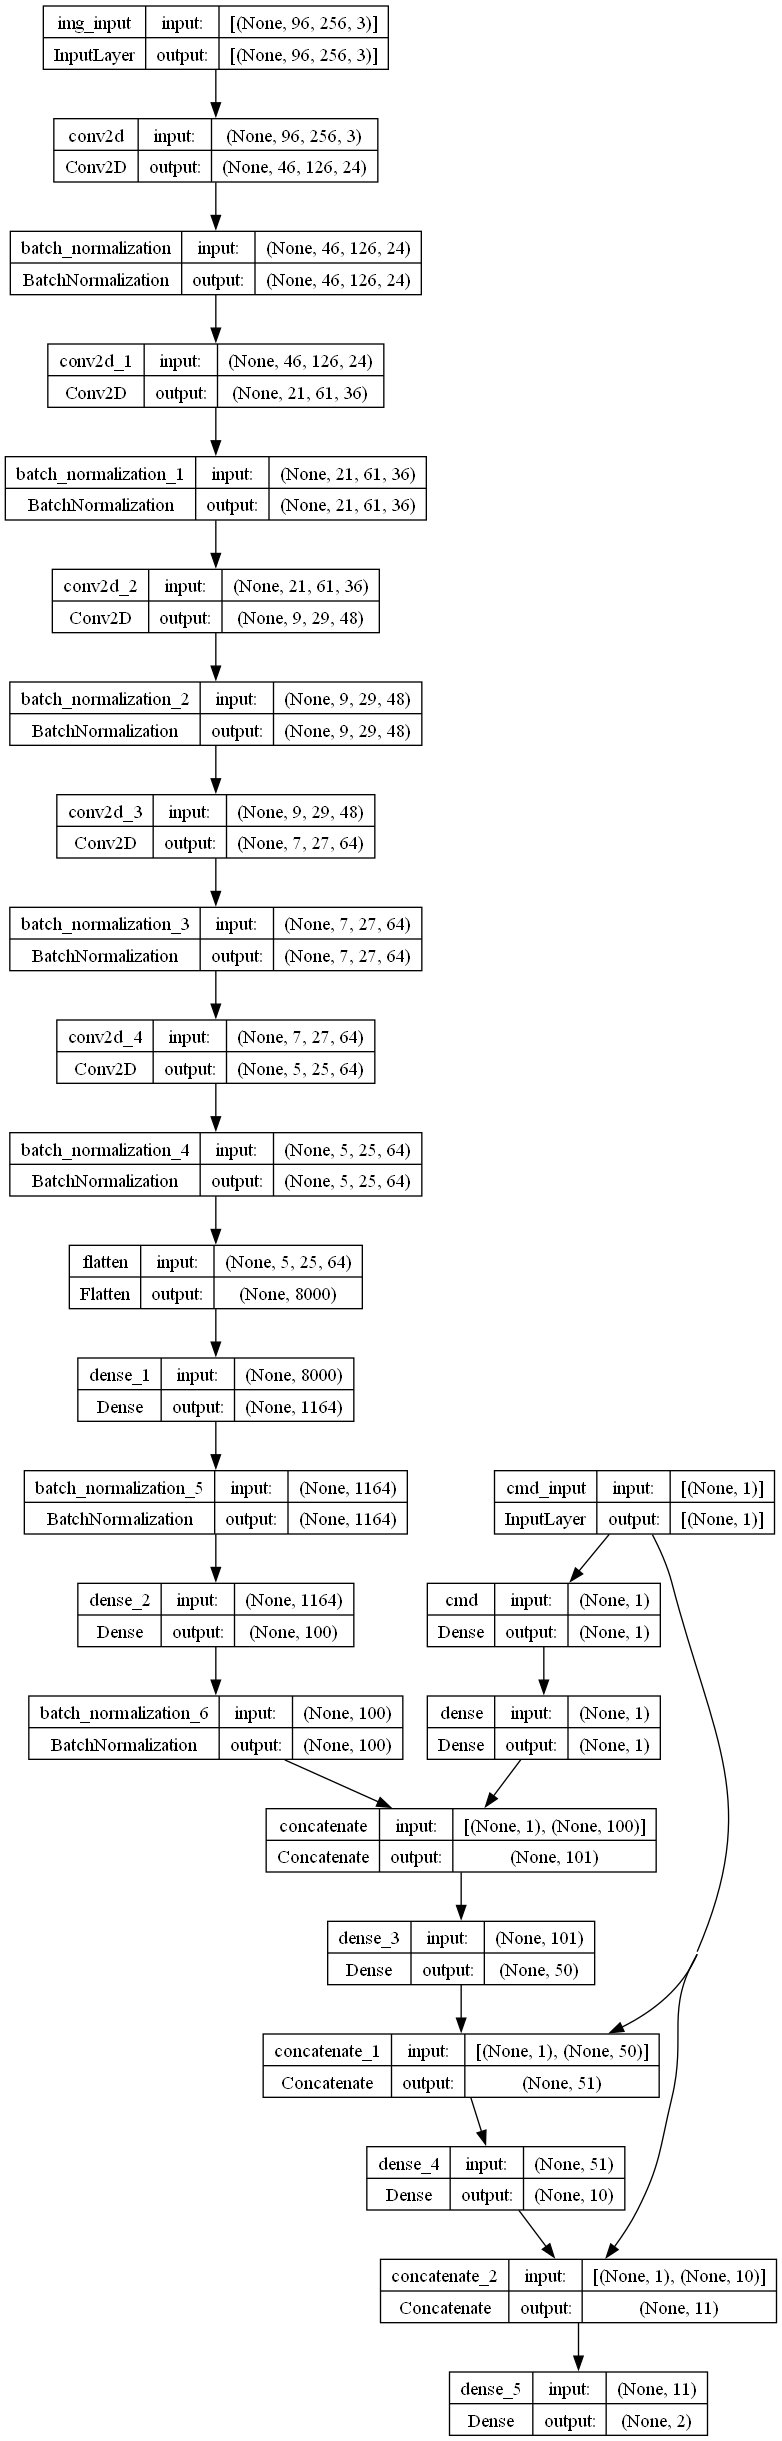
\includegraphics[width=11cm, height=20cm]{cnn_model.png}
\insertfigure{th}{0\textwidth}{cnn_model1.png}{Diagram of the Deep Learning model used in this experiment, obtained using tensorflow's plot\_model.}{fig:cnn}

There are 5 convolutions with batch normalization for the images followed by 2 Dense layers to reduce the input from 8000 to 100. Then the command inputs are concatenated with the information from the images, followed by 3 Dense layers to reduce the input from 101 to 2. All layers use "relu" as activation layers except the last that uses the linear activation function.

\subsubsection{Loss Function}

The determination of the loss function underwent adjustments through trial and error. Initially, the cumulative sum of rewards and the Mean Squared Error (MSE) \ref{eq:MSE} between $y_{true}$ and $y_{pred}$ were employed. However, difficulties appeared as the sum of rewards increased with the addition of new data, particularly when striving for unbalanced rewards, predominantly positive. This complexity in weighting led to hardships and resulted in the poor training of models.

A decision was made to transition to the mean of the rewards (MoR) \ref{eq:reward}, with the objective of maximizing it, noting that it would never surpass 15—the maximum reward possible. Yet, a subsequent challenge emerged. Minimizing the raw difference between prediction and true values resulted in models that overfit and overly generalized decisions.

Contrary to the initial approach, the original OpenBot model adopted a different strategy, focusing on the angle \ref{eq:angle} rather than the raw difference. By subtracting the command from the left motor from the command from the right motor, a negative value indicated a right turn, and vice versa. Additionally, this approach approximated the sharpness of the turn, with higher absolute values suggesting a sharper turn. This ensured that, even with variations in the robot's speed, the turn remained consistent with expectations.

Replacing the MSE of the raw values with the MSE of the angle value yielded promising results. However, in situations where both motors had identical values, the model opted to assign 0 as the value for each motor, as the difference was inherently the same: 0. Finally, the determination of the loss function was accomplished by integrating both raw values and the angle, as outlined in \ref{eq:loss}. The mean of the rewards is subtracted as the expectation is to get the loss to a minimal value while maximizing the rewards. All three have weights that can be tweaked for optimal results, in this experiment, the final weights were 1 for the MSEs and 0.8 for the rewards.

\ref{eq:loss}. 
\begin{equation}
\label{eq:angle}
\text{angle} = motor_{left} - motor_{right}
\end{equation}

\begin{equation}
\label{eq:MSE}
\text{MSE} = \frac{1}{n} \sum_{i=1}^{n} (y_{true} - y_{pred})^2
\end{equation}

\begin{equation}
\label{eq:reward}
\text{MoR} = \frac{1}{n} (\sum_{i=1}^{n} r_n)
\end{equation}

\begin{equation}
\label{eq:loss}
\text{loss\_function} = w_{MSE} \cdot MSE_{Angle} + w_{MSE} \cdot MSE_{Raw} - w_{MoR} \cdot MoR
\end{equation}

\section{Experiment Design}
\subsection{The circuit}
\label{sub:circuit}

The circuit is simple and can be seen in \ref{fig:circuit}, it makes a loop and consists of white tape placed on the ground. It is easily drivable using the controller in the medium speed setting. The floor can be slightly slippery, which can result in the robot making sudden sharp turn when asked to turn slightly. The floor is also reflective, meaning daylight can make it shine quite white, even though the human eyes can easily notice the difference, it is more difficult for a computer program with only pixel values. With the phone mounted close to the ground, figure \ref{fig:phone} shows what the phone sees.

\insertfigure{th}{0.5\textwidth}{circuit.jpg}{Picture of the circuit for this experiment. Sometimes with the table and pet cushion, sometimes without.}{fig:circuit}
\insertfigure{th}{0.5\textwidth}{phoneview.jpeg}{Picture of the circuit from phone mounted on OpenBot, with a resolution of 256*96.}{fig:phone}

\subsection{Steps to conduct experiment}
\label{sub:step}
\subsubsection{Experiment with Reinforcement Learning}
\begin{enumerate}
    \item \textbf{Setup: } Turn on the python server following the guide in the OpenBot github \cite{bib:git_openbot}. Make sure the phone and computer are connected to the same network and the OpenBot app connects to the server. Note: Verify that the phone is not in 'Lock Orientation' mode.
    \item \textbf{Initial samples: } To speed up the time-consuming process, a small number of correct laps are taken initially. This method helps improve exploration by reducing excessive randomness.
    \item \textbf{Train first model: } Train a first model with the data, name it 'reinforcement\_learning' and upload it to the OpenBot app
    \item \textbf{Initiate Exploration: } Begin by uploading the trained model and use it for exploration. Issue a negative reward from the controller when the vehicle deviates from the lane, and issue a positive reward when the vehicle remains close to the lane. If the vehicle deviates excessively, halt the exploration, reposition the robot onto the lane, and start again. The controller can still compel the robot to approach the track while in autopilot. This phase demands considerable time and requires the undivided attention of the supervisor. Continue until enough data is gathered to update the model.
    \item  \textbf{Update the model: } Move the collected data to their corresponding repository, most should go into training. Launch the notebook for training the model\ref{subsub:notebook}. Upload the updated model to the OpenBot app. Note: To avoid losing all progress with a faulty new model, it is good practice to save the previous model, especially if it is showing promising result.
    \item \textbf{Repeat: } Repeat step 4 and 5 until obtaining a satisfactory result or determining that the process is unsuccessful.
    
\end{enumerate}
\subsubsection{Experiment with traditional Machine Learning}
\begin{enumerate}
    \item \textbf{Setup: } Turn on the python server following the guide in the OpenBot github \cite{bib:git_openbot}. Make sure the phone and computer are connected to the same network and the OpenBot app connects to the server. Note: Verify that the phone is not in 'Lock Orientation' mode.
    \item \textbf{Data collection: } Collect approximately 20 minutes of data of the robot making laps. For better results, take more at different times of day and weather.
    \item \textbf{Train the model: } Move the collected data to their respective directory. Keep the best data for testing, and delete all folders with poor data. Train the model using 'pilot\_net' as model.
    \item \textbf{Upload the model: } Upload the new model to the phone. Use it with autopilot and see how it performs.
\end{enumerate}

\subsection{Security Measures}
\label{sub:security}

Given that the training is conducted on real hardware, ensuring the safety of the environment and robot is crucial. To prevent potential accidents, a mechanism has been implemented to halt the robot's movements promptly. This safety measure involves forcibly stopping the robot whenever data collection in autonomous driving is discontinued.

The initiation and termination of data collection are facilitated by a remote controller, with the action of stopping the robot triggered by pressing the designated button, R1. This manual intervention provides a layer of security, allowing immediate response and control to mitigate any unforeseen risks during the experimental process.

\section{Implementation}
\subsection{Designing the Reward Function}
\label{sub:Designing_the_reward_function}
\subsubsection{Introduction to the Reward Function}
The reward function is a fundamental component in RL, serving as the backbone for directing an agent's decision-making process in a given environment. Essentially, this function rates the consequences of an agent's actions by assigning numerical values, representing either positive or negative reinforcements.
Designing an effective reward function requires to find balance between short-term accomplishments and long-term goals. Consequently, the formulation and refinement of the reward function significantly impact the success of the reinforcement learning algorithm. 


\subsubsection{The Reward Function in the Lane Following Scenario}
In this case, the goal is to have the robot follow a lane marked on the ground. A straightforward approach involves a basic reward function, assigning positive numerical values when the robot remains on the line and negative values when it deviates. However, this simplistic setup poses a challenge: what if the robot learns that staying stationary yields the most rewards? To counter this, the system can either assign a positive reward when the robot is in motion or impose negative rewards when no command is given. Another alternative is manual rewarding, where a supervisor can press a button on the controller to administer positive or negative feedback during training, as deemed appropriate.


\subsubsection{How the Reward Function was Implemented}
Due to limited experience in JavaScript programming, the decision was made to develop and fine-tune the reward function using OpenCV in Python, analyzing images captured at different times of the day. The outlines of the detected lane and its centroid were obtained.


Following this, a simple Android application was created using Android Studio, where OpenCV was integrated as a library as seen in \ref{sub:Integration_of_OpenCV_Library}. The interface was designed to display the lane contours and centroid, alongside the centroid's distance from the expected central position. Once the functionality of the application was successfully verified, the decision was made to incorporate it as a feature within the OpenBot app, utilizing the method described in \ref{sub:Implementation_of_New_Features}.


The calculated centroid position is then compared to an ideal one. This distance is used to determine the reward. The reward $r$ can take the following values:
$$r = [-15, -1, 1, 10, 15]$$
With $-15$ and $15$ negative or positive feedback from the supervisor.


\insertfigure{th}{0.8\textwidth}{lane_detec.png}{Display of photos before and after processing to detect the lane to follow. On the left is displayed the ideal result of lane detection. On the right is example on how the luminosity impacts the result and could be problematic}{fig:lane_detec}

On the upside, the computation for this reward function is lightweight and integrates with the standard data logging process without issues. The calculation is performed directly on the smartphone and is transmitted alongside other sensor data, including images, command value logs, and accelerometer readings.



However, there are downsides to consider. Firstly, the reward function's applicability is limited to the specific circuit. Additionally, its sensitivity to variations in light sources, time of day, and weather conditions can lead to inconsistent performance as seen in \ref{fig:lane_detec}. To avoid detecting white from objects on the wall or furniture, only the bottom 20\% of the picture is taken into account. There are instances where the function fails to detect the lane even when it is clearly visible, which can be problematic during the model training phase. And a bad reward function can potentially hinder the learning process and affect the model's performance.

\subsection{Modification of the OpenBot app}
\label{sub:Modification_of_openbot}
\subsubsection{Logger Fragment}

The reward function from \ref{sub:Designing_the_reward_function} was implemented directly in the Logger Fragment of the OpenBot app, which means it was calculated while the model is running and the data is collected. In the $processFrame$ function, the OpenCV processing is applied to the same bitmap (image) as the frame collected and the processed image is then saved to a new folder. These images are just to ensure the processing goes as planned and are not used in the model. 
\\[3mm]
Here is the detail of how the image is processed using OpenCV:
\begin{enumerate}
    \item Conversion to grayscale
    \item Addition of contrast to the image with a factor of 1.2.
    \item Normalization of the image values to a range between 0 and 255 after contrast adjustment.
    \item Detection of white pixels using trial-and-error determined lower and upper bounds of $[200,170,170]$ and $[254,254,254]$, respectively.
    \item Application of median blur with a factor of 9 to the image.
    \item Utilization of the $Canny$ function from OpenCV in JavaScript to obtain edges.
    \item Retention of only the Region of Interest, specifically the bottom 20% of the image.
    \item Calculation of the centroid, with only the x-value considered in computing the reward function.
\end{enumerate}


\noindent The processed images are showed in \ref{fig:lane_detec}. 
\\[3mm]
Following the code from the Autopilot Fragment and pre-existing code in the Logger Fragment, adding the necessary functions such as $startAutonomousDriving$, $stopAutonomousDriving$, $handleDriveCommandAutonomous$ and $processFrameForAutonomous$,  are pretty straightforward. There are also the functions to change the reward to +15 or -15 using the command inputs from the controller and the function changing the reward using the distance between the calculated centroid position and the ideal centroid position. Refer to the appendices \ref{sub:log} for more details on the code.


\subsubsection{Log Data Utils and Sensor Service}

The information from the Logger Fragment passes through the Log Data Utils to turn into a Message with the right format for the Sensor Service: 
\begin{lstlisting}
  public static Message generateRewardMessage(long reward){
    Message msg = Message.obtain();
    Bundle bundle = new Bundle();
    bundle.putLong("rewardNumber",  reward);
    bundle.putLong("timestamp", SystemClock.elapsedRealtimeNanos());
    msg.setData(bundle);
    msg.what = SensorService.MSG_REWARD;

    return msg;
  }
\end{lstlisting}

In the Sensor Service script, a path to create the reward folder is necessary, then, the .txt file also needs to be created. Each new reward received during the data collection is added to this text file. Once the data collection is finished, the .txt file is closed as well as the folder. To do so, following the example of the other logged data is quite intuitive.



\subsection{Presentation of the Python Scripts}
\label{sub:python}
There are 12 different python scripts to process the data and train the models. There are also 10 scripts for the python server used for transmitting data from OpenBot to the computer, however, they were not modified because of a lack of knowledge in Python servers programming. Finally, there is a notebook in the .ipynb format for running all the scripts and training the models. 

Here is a list of the 12 python scripts and what they do:
\begin{itemize}    
    \item \textbf{\_\_init\_\_:} This script establishes the necessary project structure and ensures the existence of essential directories for storing data and models.
    \item \textbf{associate\_frames:} The script ensures synchronization between frames and control signals as well as frames and rewards, facilitating further analysis and training of machine learning models.
    \item \textbf{callbacks:} The callbacks offer flexibility and functionality for optimizing and monitoring the training of neural network models. They can be employed based on specific requirements during the training process.
    \item \textbf{data\_augmentation:} This script contribute to enhancing the diversity of the training dataset, which can improve the generalization and robustness of machine learning models trained on the data. However, it is not adapted to take into account rewards.
    \item \textbf{dataloader:} This class is designed to simplify the process of accessing labeled data for training neural network models. It provides functionalities for loading labels, rewards, building lookup tables, and efficiently retrieving labels and rewards based on file paths.
    \item \textbf{losses:} This script regroups all the loss functions.
    \item \textbf{metrics:} These metrics are designed to evaluate the performance of models in predicting angles, specifically focusing on the absolute difference and the correct direction of the angles. They can be used during model training to monitor how well the model is capturing the desired angle-related behaviors.
    \item \textbf{models:} This script regroups all the available models for training.
    \item \textbf{tfrecord:} The script is used to generate TensorFlow Record (TFRecord) files from a collected dataset. These TFRecord files are a more robust and efficient way of loading data for training a driving policy. 
    \item \textbf{tfrecord\_utils:} This script provides utility routines for manipulating TensorFlow records (TFRecords).
    \item \textbf{train:} The train script is a training script for a neural network using TensorFlow. It includes components for handling data in both directory format and TFRecord format, as well as training and evaluation procedures. The script can be configured to train different models (specified in the --model argument) with various hyperparameters. Additionally, it supports loading data either from directories or TFRecord files, and it provides an option to create TFRecord files from the raw data.
    \item \textbf{utils:} This script includes utility functions for working with TensorFlow and some related libraries. These utilities cover a range of tasks related to machine learning and deep learning workflows. 
\end{itemize}

\subsection{Preprocessing of the Data in associate\_frames.py}
\label{sub:preprocessing}

By applying a the same procedure to link frames with corresponding control commands, the rewards have to be handled in the process. Two new files are created in the process using the original 'rewardLog.txt' file: 'matched\_frame\_reward.txt' and 'matched\_frame\_reward\_processed.txt'. 

The association between frames and rewards is established by matching their corresponding timestamps. Although these timestamps are in nanoseconds and rarely identical, calculating the timestamp difference generates the 'matched\_frame\_reward.txt' file, labeled with 'timestamp (frame), time\_offset (reward-frame), frame, reward'. Only when the offset is below a specified threshold are the reward and frame considered associated. The file can undergo further processing, eliminating unwanted values like zeros or NaN, if necessary. However, in this context, all numerical values are retained. The resulting processed file has for labels 'timestamp, frame, reward'. Associating the frames to their corresponding commands and reward is a crucial step for model training. To see the code, please refer to the appendices \ref{sub:associate}.



\subsection{Adding Rewards to the Dataloader and tf records}
\label{sub:reward}
Integrating rewards into the dataloader or TF records mirrors the process for adding labels, already implemented in the original script. It's crucial to adjust the path to the reward file in the following manner:
\begin{lstlisting}[language=Python]
            ...
                    rewards_file = os.path.join(
                        data_dir,
                        dataset,
                        folder,
                        "reward_data",
                        "matched_frame_reward_processed.txt",
                    )
                    print("reward_file", rewards_file)
            ...  
\end{lstlisting}

The remaining part of the function responsible for retrieving rewards should use this updated path. Additionally, the function should return a dictionary where each frame serves as the key, paired with its corresponding reward.

\subsection{Modification of the train.py Script}
\label{sub:mod_train}
In the train.py script, when calling data from the dataloader or tfrecord, introduce the reward as a new feature in the label:

\begin{lstlisting}[language=Python]
    ...
        label = [features["left"], features["right"], features["reward"]]
    ...
\end{lstlisting}

Maintain uniformity in the number of features for each label, by comparing the frames in rewards and the commands and only keeping the common ones, as demonstrated in the appendices \ref{sub:train}.

In order to use the custom loss seen in \ref{sub:Choice_of_model}, an if statement needs to be added as follows:

\begin{lstlisting}[language=Python]
if tr.hyperparameters.POLICY == "autopilot":
        tr.loss_fn = losses.sq_weighted_mse_angle
    elif tr.hyperparameters.POLICY == "point_goal_nav":
        tr.loss_fn = losses.mae_raw_weighted_mse_angle
    if tr.hyperparameters.MODEL == "pilot_reinforcement":
        tr.loss_fn = losses.custom_loss
\end{lstlisting}

\subsubsection{Adapting the policy\_learning.ipynb notebook}
\label{subsub:notebook}
This notebook plays a crucial role in training and visualizing data, including the training process and resultant graphs. To adapt the notebook for use with the reinforcement learning model, follow a few essential modifications. Firstly, set the desired model:

\begin{lstlisting}[language=Python]
params.MODEL = "pilot_reinforcement"
\end{lstlisting}

Ensure the variable no\_tf\_record is set to False. This adjustment addresses an unresolved issue with the original code's dataloader, which seems to duplicate a unique command and reward multiple times:

\begin{lstlisting}
no_tf_record = False 
\end{lstlisting}

Given the potentially extensive training duration, using a GPU with CUDA support is strongly recommended. A CUDA version of 11.3 is optimal, ensuring compatibility with other libraries.

Once the training is complete, the model is then saved in the .tflite format within the 'models' folder. Note that if the new model shares its hyperparameters with a previous one, it automatically replaces the older model.

\newpage
\subsection{Python Server for Data Transmission}
\label{sub:server}
The Python server assumes an important role in ensuring the flow of data between the robot and the computer, acting as a central hub for all activities related to model training. The process involves the robot transmitting compiled data to the server. The ensuing folder, containing the datasets, is stored in the designated 'uploaded' directory. This folder features a preview option seen in fig \ref{fig:preview} and the users can relocate it to either the training or testing directory, or delete it in case of issues.

\insertfigure{th}{0.5\textwidth}{preview.png}{Preview of the data collected with pictures flashed consecutively like a video, the option to move directory is also displayed as 'Actions'.}{fig:preview}


Following the completion of model training, the server recognizes the model in tflite format, this can be seen in figure \ref{fig:model}. This registered model, customizable with a user-specified name, can be uploaded to the OpenBot app as seen in figure \ref{fig:uploading}. It's important to note that assigning an existing model name will replace the older model with the most recently trained iteration.

\insertfigure{th}{0.4\textwidth}{model.png}{Screenshot of the server's model uploading scheme. The same model can be uploaded multiple times under different names and uploaded models can be deleted.}{fig:model}

\insertfigure{th}{0.4\textwidth}{uploading.png}{Screenshot of the models details, the model is uplaoded to the OpenBot app by clicking the 'Push to Phone' button.}{fig:uploading}

\newpage
\section{External tools used in the making of this thesis}
Following is a list of tools and websites that helped in the research and writing of this thesis:
\begin{itemize}
    \item \textbf{TensorFlow \cite{bib:TensorFlow} library and websites: } There are lots of documentation on how to correctly use tensorflow and adapt it to a specific scenario. This was very important to understand the pre-existing scripts and how to implement the reinforcement learning part.
    \item \textbf{CUDA websites and online guides \cite{bib:CUDA} } Installing the correct version of CUDA can be challenging with all the possible resulting conflicts from installing a version incompatible with the different owned libraries. Online guides and the CUDA website helped tremendously and allowed to accelerate the training to up to 10 times faster.
    \item \textbf{Python's and JavaScript's \cite{bib:javascript} community: } Luckily there are lots of documentation online to help programming in Python and JavaScript. They were crucial to the understanding of the current scripts as well as a great help to implement the new libraries, such as OpenCV on Android Studio.
    \item \textbf{DeepL Write beta\cite{bib:DeepL}, ChatGPT \cite{bib:chatGPT} and Thesaurus \cite{bib:thesaurus}: } These helped with the writing of this thesis. DeepL Write is also in beta testing to help improve written sentences and was used to help formulating clearer sentences. Figure \ref{fig:deepl} shows how it was used, for instance on the text just above. Thesaurus was used to find synonyms of overutilized words such as 'difficulties' and 'challenge'. Finally, ChatGPT was also able to provide some guidance in structuring this thesis, helping with making understandable and concise section and subsection titles. It also provided guidance in writing the Conclusion \ref{sub:Conclusion} with guidelines of what it should contain. All the research done in this thesis and ideas are personal, these AI were used to assist in the formatting and grammar. Here is an example of how it was used: 
\end{itemize}

\textbf{User: } \textit{How long should a conclusion of a master thesis be ?} \\
\vspace{5pt}

\textbf{ChatGPT 3.5: } \textit{The length of the conclusion in a master's thesis can vary depending on factors such as the overall length of the thesis, the complexity of the research, and the specific requirements of the academic institution. However, there are some general guidelines you can consider:
Proportionality: As a rough guide, the conclusion typically constitutes about 5-10\% of the total thesis length. If your thesis is 100 pages long, the conclusion might be around 5-10 pages.
Summarize Key Points: The conclusion should provide a concise summary of the key points discussed in the thesis. It's an opportunity to remind the reader of the main findings and contributions of your research.
Answer Research Questions/Objectives: Clearly state how your research has addressed the research questions or objectives outlined in the introduction. Discuss whether your findings support or refute your initial hypotheses.
Implications and Contributions: Discuss the broader implications of your research and its potential contributions to the field. This could involve discussing practical applications, suggesting areas for future research, or highlighting the significance of your findings.
Limitations: Acknowledge any limitations of your study. Every research project has limitations, and it's important to address them in the conclusion to provide a balanced view of your work.
Concluding Thoughts: End the conclusion with some final thoughts that tie everything together. You might also discuss the importance of your research in the larger context of your field.
Remember, these are general guidelines, and the specific requirements for your master's thesis may vary. It's always a good idea to consult the guidelines provided by your academic institution or department and seek guidance from your advisor. Additionally, consider the expectations for conclusions in your specific field of study, as requirements can vary across disciplines.}


\insertfigure{th}{1\textwidth}{DeepL.png}{Screenshot of an example for DeepL's usage in sentence enhancement.}{fig:deepl}
%%=== chapter: results ===
\chapter{Results}
\label{sub:Results}
In this chapter the results from the described method are given,  as well as results on the same task using the standard method, expected for OpenBot.
%%=== section: results 1 ===
\section{Results using Reinforcement Learning}
\label{sub:results_rl}
\subsection{Training Performance}

Initially, the steps outlined in subsection \ref{sub:step} were followed. Approximately 5 minutes of data were collected, 3 minutes for training and 2 minutes for testing. The first model, named 'reinforcement\_learning', was trained and uploaded. The model ran and continuously collected data until it deviated significantly from the circuit, resulting in significant negative rewards (-15). Manual intervention was required to bring the robot back on track.

Every two minutes of data collected triggered an update of the model. It took approximately 6 to 7 updates before any noticeable progress was made in decision making. Due to the predominance of left or right turns in the laps, the model struggled to turn in the less common direction. Guiding the robot, imposing penalties for undesirable behaviour and selectively adding data to address incorrect decisions helped to mitigate this problem.

However, an unresolved challenge remained - the robot would continue straight ahead if it lost sight of the track, posing a safety risk and cost times with bad data collection. 

\subsection{Task Performance}

The conclusive model demonstrated the capability to follow the lane and complete up to 4 laps before losing track. The model exhibited close adherence to the lane and appeared to decelerate during turns. Challenges arose, particularly on the side of the circuit closer to the windows, where the likelihood of losing track and discontinuing turns was notably higher.

\subsection{Time Efficiency}

Achieving successful laps required about 30 minutes of data, but training from scratch took a total of 8 to 10 hours. 

\subsection{Sensitivity Analysis}

As previously noted, the model encountered difficulties in areas illuminated by natural white lighting, affecting the robot's behavior. Additionally, the robot exhibited slight susceptibility to specific changes; for instance, adjusting the position of a red handbag led to the robot missing a turn. However, the removal of a wooden box or a chair did not appear to have a discernible impact on the model.


%%=== section: results 2 ===
\section{Results using traditional Machine Learning}
\label{sub:results_ml}
\subsection{Training Performance}
Continuing with the procedures outlined in subsection \ref{sub:step}, a total of approximately 20 minutes of data was collected, focusing on retaining only high-quality data without significant deviations from the lane. The model underwent training using the Python Server and was subsequently uploaded to the phone. Noteworthy challenges were minimal in this phase, with the exception of occasional ground slipperiness leading to the potential obsolescence of longer runs of data collection. 

\subsection{Task Performance}

The machine learning model exhibited the capability to complete up to 7 laps before deviating too significantly from the lane and encountering obstacles. Interestingly, the model did not consistently rely on the lane as a guideline but rather seemed more attuned to details from the surrounding decor. While successfully navigating all turns, the model spent minimal time on the lane itself. Notably, the performance of the model was highly contingent on various lighting conditions and weather.

\subsection{Time Efficiency}

The entire process of data gathering and model training took approximately 2 hours. Notably, the familiarity with the circuit significantly contributed to the success of data gathering time efficiency.

\subsection{Sensitivity Analysis}

As previously highlighted, the traditional model demonstrated sensitivity to various lighting sources. To mitigate this, data collection was conducted at different times of the day and on diverse weather conditions. The model also exhibited high susceptibility to moving objects, such as a cat entering the scene

%%%%%%%%%%%%%%%%%%%%%%%%%
%%=== chapter: analysis ===
\chapter{Analysis and Discussion}
\label{sub:Analysis_and_discussion}
In this chapter, the results are analysed, compared and some perspective is given concerning future steps to improve the Reinforcement Learning method.

%%=== section: analysis 1 ===
\section{Analysis of Reinforcement Learning with OpenBot}
\label{sub:analysis_rl}
\subsection{Inefficiencies and Unusual Behaviors}
The obtained results are promising although showcase some inefficiencies, manifesting in strange behaviors that prove challenging to rectify. A notable issue arises when the vehicle loses sight of the lane. Instead of actively attempting to rediscover the lane, the model tends to persistently move forward. This behavior significantly impacts the exploration and learning phases, leading to repetitive occurrences that pose a considerable challenge. Rectifying this behavior solely by relying on inputs where such issues are absent proves to be very time-consuming. This issue occurs because the robot  keeps moving while gathering data, when lost, it does what is the most rewarding in the majority of situations, moving straight ahead.

\subsection{Unlearning capabilities}

As previously mentioned, unlearning a bad behavior can prove to be quite challenging in Reinforcement Learning. However, in this scenario, all the data gathered is kept and can be removed when updating the model. If the datasets behind the problematic behaviors can be pinpointed, then, they can be removed and the updated model will produce better results. This happened when the car started to skip a turn and go straight since further down, the lane reappears. After removing the problematic behavior from the dataset used in training, the robot stopped doing it.

\subsection{Response to Updated Models}

Another observation is the variability in the robot's behavior between updates, indicating that the robot is consistently acquiring new knowledge after each update. However, this variability can also be attributed to the randomness in training and validation sets. Training the model twice with the same datasets and hyperparameters can provide slightly different results.

\subsection{Sensitivity to Lighting Conditions}

A critical factor contributing to the model's poor performance is the high dependence on lighting conditions in reward computation. The RL model's sensitivity to varying illumination levels introduces a significant source of inconsistency, impacting its reliability across diverse environmental settings.

\subsection{Loss Function and reward Design}

Another important factor influencing the observed limitations is the sub-optimal design of the loss function. The current formulation fails to capture essential nuances, hindering the model's ability to learn effectively. Additionally, the more data is captured, the more rewards there is and individual rewards such as the inputs of the supervisor have less impact overall. 

%%=== section: analysis 2 ===
\section{Analysis of traditional Machine Learning}
\label{sub:analysis_ml}
\subsection{Adaptability and Light Conditions Dependency}
The traditional Machine Learning model, intended with OpenBot, showcases adaptability, successfully completing laps following thorough data gathering. Nevertheless, its performance is highly dependent on lighting conditions, displaying sensitivity to alterations in weather, time of day or shadows. 

\subsection{Response to Object Movement and Unpredictable Behaviors}

The model's sensitivity to the changes of objects' positions and unexpected scenarios is evident. Instances where objects move or the sudden appearance of a cat behind the robot can induce unusual behaviors, such as skipping turns and proceeding straight. These peculiar responses highlight the model's susceptibility to unforeseen elements in its surroundings.

\subsection{Efficient Training and Intuitiveness}
The training process for traditional Machine Learning is time-efficient, conducted directly on the server. Moreover, the method is considered very intuitive, offering a user-friendly training process.

%%=== section: analysis conclusions ===
\section{Comparison of the two methods}
\label{sub:compare}
The comparison between the reinforcement learning (RL) and machine learning (ML) methods reveals distinct strengths and challenges associated with each approach. In terms of lane following performance, the RL method demonstrates a higher level of interest and proficiency in adhering to the lane. This is attributed to its supervised training, where only the most effective data—instances where the robot stays on the lane—are utilized for training. Additionally, the inclusion of a substantial punishment for veering off the lane (-15) contributes to the improved lane-following behavior of the RL model. On the other hand, the ML method, while capable of completing laps, tends to deviate from the lane. This behavior shows that the model does not focus on the lane to make its decision, but more likely to the general surroundings. 

In terms of time efficiency, autonomy, and intuitiveness, the ML method outperforms RL. The ML approach gathers data in a single run and trains the model, with the option to collect additional data for specific challenges. Furthermore, the training process is notably less time-consuming, particularly when GPU support is unavailable. In contrast, the RL method demands constant attention during training, involving multiple steps such as uploading the model and frequent small updates, resulting in a more time-intensive process. The autonomy and intuitiveness of the ML method currently surpass those of RL.

Both methods exhibit sensitivity to light, albeit for different reasons. The ML method tends to overfit to given data, making it challenging to handle variations in object positions or lighting conditions. Meanwhile, the RL model faces issues with the reward function's sensitivity to light, potentially leading to errors in reward assignment. Despite this sensitivity, the RL method holds theoretical robustness compared to ML when trained appropriately.

Concerning unwanted behaviors and learning, the RL method carries a higher risk of learning undesirable actions. For instance, it may send insufficient motor values, making the robot stand still, while still collecting positive rewards for staying on the lane. On the other hand, the ML method may exhibit unwanted behaviors due to overfitting, although it might be less prone to specific issues encountered by RL.

In conclusion, both RL and ML methods showcase capabilities in completing the circuit, each with its strengths and challenges. RL proves to be more efficient in lane following, while the simplicity and efficiency of the ML method provide advantages in terms of time, autonomy, and intuitiveness.


\section{Important notes}

There are two testing methods for model evaluation: the traditional Autopilot feature and running the model during data gathering for semi-online reinforcement learning. Notably, there was a discernible difference in the behavior of the same models under these two scenarios. The computational demands during data gathering potentially hindered the model's decision-making, leading to varied behavior.

It was consistently verified that the same model ran in both situations. However, for both RL and traditional machine learning models, the Autopilot feature showcased better behavior. Final testing for both models was conducted using Autopilot. Interestingly, the RL model demonstrated superior results in the running-during-data-gathering scenario, possibly attributed to its predominant training and evaluation using this method.

An additional note concerns the impact of moving objects on model results. Objects were not deliberately moved; however, as the results were collected over several days in a residential environment, their movement was incidental and not part of any deliberate research design.

\section{Future steps}
\label{sub:future}

In terms of future steps and potential improvements, several avenues can be explored to enhance the performance and educational aspects of the project. One key focus is on refining the reward function. One suggestion involves training a dedicated machine learning model for lane detection in the specific scenario, using the validated images from the less effective reward function designed here. Once the robust model is trained, it can be added in .tflite format to the OpenBot app, providing a much more accurate reward function. Additionally, the idea of creating a more traditional reinforcement learning model from scratch, with a stronger focus on the reward, offers a promising direction for further exploration. This approach would involve developing a model that relies more on reinforcement learning principles than the initial implementation, potentially addressing limitations in the current reward function.

To address time efficiency concerns, the implementation of a resetting function is proposed. This function could utilize external sensors or an algorithm designed to reposition the robot on the lane when it deviates too far. The goal is to minimize the need for constant human supervision and intervention during the training process.

In terms of educational improvements within the OpenBot Platform, it is suggested to enhance the design of implemented features. Creating dedicated spaces for components such as the reward function within the platform can simplify the learning process for future students. Improving the server infrastructure to support training directly within the platform, enhancing Python scripts for clarity, and facilitating direct comparison between traditional machine learning and reinforcement learning methodologies can contribute to a more accessible and effective educational experience.

Expanding the application of this work to other educational robots, such as the Donkey Car or TurtleBot, offers the opportunity to implement reinforcement learning in diverse educational settings. This approach would enable students to gain insights into the adaptability and applicability of reinforcement learning across various robotic platforms.

Looking forward, a compelling future direction involves leveraging smartphones as sensors for other robotic platforms. This approach entails collecting data from sensors on phones and transmitting it to a Python server for model training. The integration of mobile devices extends the versatility of the robotic platforms, opening up new possibilities for sensor integration and data collection in educational settings.

In conclusion, these future steps and improvements aim to advance both the technical capabilities and educational value of the project, offering valuable insights into reinforcement learning and robotics for students.

%%=== chapter: summary (original language) ===
\chapter{Conclusion and future Perspective}
\label{sub:Conclusion}
In conclusion, this thesis has undertaken a thorough exploration of reinforcement learning (RL) and traditional machine learning methodologies within the context of the OpenBot platform. The focal point was the comparative analysis of their effectiveness in data gathering and circuit navigation, particularly in the challenging scenario of lane following. The investigation has provided valuable insights into the nuanced strengths and challenges associated with both RL and machine learning methods.

One notable revelation from this study is the superior lane-following performance demonstrated by the RL method. This superiority can be attributed to the meticulous supervision and curation of training data, which allowed the RL model to showcase a heightened interest in adhering to the lane. The incorporation of a substantial punishment for deviations from the lane further contributed to the robustness of the RL model in this specific scenario.

However, a crucial consideration emerged concerning time efficiency, autonomy, and intuitiveness. The machine learning method exhibited superiority in these domains, presenting a simpler and more streamlined process. The ML approach, capable of gathering and training on data efficiently in a single run, outperformed the RL method, which demanded constant attention during training and involved a more intricate, time-consuming process.

As we turn our gaze toward the future, several avenues for improvement and expansion have been identified. Enhancements to the reward function, including the integration of a dedicated machine learning model for lane detection, hold promise for increased accuracy and effectiveness. The proposal of a resetting function to minimize human intervention and address time efficiency concerns signifies a practical step toward achieving greater autonomy in the learning process.

From an educational standpoint, there is a clear need for refinements within the OpenBot platform to enhance user experience. Specific design improvements, such as dedicated spaces for essential components and a more user-friendly server infrastructure, can contribute to a more accessible learning environment. Comparisons between traditional machine learning and RL methodologies, as well as the adaptation of this work to other educational robots, offer valuable opportunities for enriching educational content and experiences.

Notably, this research also underscores the feasibility of RL training with real hardware, a departure from conventional practices relying on simulated environments. While demonstrating the potential of real-world RL training, it is crucial to acknowledge that it requires constant supervision and manual resetting. This finding sheds light on the challenges associated with implementing RL in practical, hardware-based applications.

Looking ahead, the integration of smartphones as sensors for robotic platforms opens up exciting possibilities for expanding the scope of data collection and training. This forward-thinking approach represents a potential avenue for future research, extending the versatility of robotic platforms and enriching the learning experiences of students and enthusiasts alike.

In conclusion, this research not only contributes valuable insights into the practical implementation of RL in mobile robotics but also underscores the importance of considering diverse methodologies to meet specific challenges. As the field of robotics and machine learning continues to evolve, the findings presented here provide a foundation for future explorations and innovations in the realm of autonomous systems and educational robotics.
%%=== chapter: acknowledgements ===
\chapter*{Acknowledgements}
\addcontentsline{toc}{chapter}{Acknowledgements}

I extend my sincere gratitude to my family and my partner for their immense support throughout this academic journey. Your encouragement and understanding have been my pillars of strength.

\vspace{10pt}
\noindent I would also like to express my deepest appreciation to my supervisor, Naveed Muhammad, for his invaluable guidance, positivity, and reliable support. 

\vspace{10pt}
\noindent Additionally, I want to thank the University of Tartu and the Institute of Technology for making this research possible.

\vspace{10pt}
\noindent Finally, I am very grateful for Matthias Müller, who generously donated 4 OpenBot platforms to the University and allowed this research to be possible.

\vspace{10pt}
\noindent This achievement would not have been possible without the collective support and encouragement from my loved ones and mentors. Thank you for being an integral part of this rewarding experience.

\begin{figure}[h]
    \centering
    
\includegraphics[width=0.8\textwidth]{signature.png}
\end{figure}

%%=== references ===
\begin{thebibliography}{99}
%% reference to the network ressource, namely Wikipedia according to its recommendations
\bibitem{bib:openbot} 
M. M{\"u}ller and K. Vladlen, 
"OpenBot: Turning Smartphones into Robot", 
\textit{Proceedings of the International Conference on Robotics and Automation (ICRA)}, 2021, 
DOI: \href{https://doi.org/10.48550/arXiv.2008.10631}{10.48550/arXiv.2008.10631}
\bibitem{bib:git_openbot}
M. M{\"u}ller and K. Vladlen, OpenBot GitHub repository: \href{https://github.com/isl-org/OpenBot}{https://github.com/isl-org/OpenBot}
\bibitem{bib:openbotLeonLilou}
L. Glorieux, L.Gras,
"Autonomous vehicles project: OpenBot", 2022,
\href{https://medium.com/@lgopenbot/autonomous-vehicles-project-openbot-aa806fd1829c}{https://medium.com/@lgopenbot/autonomous-vehicles-project-openbot-aa806fd1829c}

\bibitem{bib:richard}
R. Bellman
"The Theory of Dynamic Programming", 1954
Link to the paper: \href{https://www.ams.org/journals/bull/1954-60-06/S0002-9904-1954-09848-8/S0002-9904-1954-09848-8.pdf}{https://www.ams.org/journals/bull/1954-60-06/S0002-9904-1954-09848-8/S0002-9904-1954-09848-8.pdf}
\bibitem{bib:delayed}
C. Watkins,
"Learning from Delayed Rewards", 1989,
Access to PDF: \href{https://www.researchgate.net/publication/33784417_Learning_From_Delayed_Rewards}{Learning from Delayed Rewards}

\bibitem{bib:Tesauro}
G. Tesauro,
"Temporal difference learning and TD-Gammon"
\textit{Communication of the ACM Vol.38, No.3}, 1995
DOI: \href{https://doi.org/10.1145/203330.203343}{10.1145/203330.203343}

\bibitem{bib:deepmind}
V. Mnih, K. Kavukcuoglu, D. Silver, A. Graves, I. Antonoglou, D. Wierstra, M. Riedmiller,
"Playing Atari with Deep Reinforcement Learning"
\textit{arXiv:1312.5602v1 [cs.LG]}, 2013,
Link to the paper: \href{https://arxiv.org/abs/1312.5602}{https://arxiv.org/abs/1312.5602}
\bibitem{bib:omnidirectional}
R. Hafner and M. Riedmiller,
"Reinforcement Learning on an Omnidirectional Mobile Robot",
\textit{Proceedings 2003 IEEE/RSJ International Conference on Intelligent Robots and Systems (IROS 2003) (Cat. No.03CH37453)}, 2003,
DOI: \href{https://doi.org/10.1109/IROS.2003.1250665}{10.1109/IROS.2003.1250665}
\bibitem{bib:NRL}
R. Hafner and M. Riedmiller,
"Neural Reinforcement Learning Controllers for a Real Robot Application",
\textit{Proceedings 2007 IEEE International Conference on Robotics and Automation}, 2007,
DOI: \href{https://doi.org/10.1109/ROBOT.2007.363631}{10.1109/ROBOT.2007.363631}
\bibitem{bib:drivesim}
P. Wolf, C. Hubschneider, M. Weber, A. Bauer, J. Härtl, F. Dürr, J. . Zöllner,
"Learning how to drive in a real world simulation with deep Q-Networks",
\textit{2017 IEEE Intelligent Vehicles Symposium (IV)}, 2017, 
DOI: \href{https://doi.org/10.1109/IVS.2017.7995727}{10.1109/IVS.2017.7995727}
\bibitem{bib:reset}
B. Eysenbach, S. Gu, J. Ibarz, S. Levine,
"Leave no Trace: Learning to Reset for Safe and Autonomous Reinforcement Learning",
\textit{arXiv:1711.06782v1 [cs.LG]}, 2017,
DOI: \href{https://doi.org/10.48550/arXiv.1711.06782}{10.48550/arXiv.1711.06782}
\bibitem{bib:walk}
T. Haarnoja, S. Ha, A. Zhou, J. Tan, G. Tucker, S. Levine
"Learning to Walk via Deep Reinforcement Learning"
\textit{arXiv:1812.11103v3 [cs.LG]}, 2019
DOI: \href{https://doi.org/10.48550/arXiv.1812.11103}{10.48550/arXiv.1812.11103}
\bibitem{bib:sarl}
K. Li, Y. Xu, J. Wang, Max Q.-H. Meng
"SARL: Deep Reinforcement Learning based Human-Aware Navigation for Mobile Robot in Indoor Environments",
\textit{2019 IEEE International Conference on Robotics and Biomimetics (ROBIO)}, 2019
DOI: \href{https://doi.org/10.1109/ROBIO49542.2019.8961764}{10.1109/ROBIO49542.2019.8961764}

\bibitem{bib:realcar}
M. Riedmiller, M. Montemerlo, H. Dahlkamp,
"Learning to Drive a Real Car in 20 Minutes",
\textit{2007 Frontiers in the Convergence of Bioscience and Information Technologies}, 2007,
DOI: \href{https://doi.org/10.1109/FBIT.2007.37}{10.1109/FBIT.2007.37}
\bibitem{bib:vtr}
L. Tai, G.e Paolo, M. Liu,
"Virtual-to-real deep reinforcement learning: Continuous control of mobile robots for mapless navigation",
\textit{2017 IEEE/RSJ International Conference on Intelligent Robots and Systems (IROS)}, 2017,
DOI: \href{https://doi.org/10.1109/IROS.2017.8202134}{10.1109/IROS.2017.8202134}
\bibitem{bib:leg}
S. Ha, J. Kim, K. Yamane,
"Automated Deep Reinforcement Learning Environment for Hardware of a Modular Legged Robot",
\textit{15th International Conference on Ubiquitous Robots (UR)}, 2018,
DOI: \href{https://doi.org/10.1109/URAI.2018.8442201}{10.1109/URAI.2018.8442201}

\bibitem{bib:alphastar}
Google DeepMind,
"AlphaStar: Grandmaster level in StarCraft II using multi-agent reinforcement learning" , 2019, Link to website: \href{https://deepmind.google/discover/blog/alphastar-grandmaster-level-in-starcraft-ii-using-multi-agent-reinforcement-learning/}{https://deepmind.google/discover/blog/alphastar-grandmaster-level-in-starcraft-ii-using-multi-agent-reinforcement-learning/}

\bibitem{bib:ai}
Achievements AI Website, on Game Artificial Intelligence, Milestone from 1992.
Link to website: \href{https://achievements.ai/}{https://achievements.ai/}

\bibitem{bib:phone}
Xiaomi, 2023, \href{https://www.mi.com/global/product/redmi-note-11/}{https://www.mi.com/global/product/redmi-note-11/}
\bibitem{bib:opencv}
OpenCV, Releases, 2023, Link for downloading: \href{https://opencv.org/releases/}{https://opencv.org/releases/}

\bibitem{bib:TensorFlow}
Google, TensorFlow, 2023,
link to website: \href{https://www.tensorflow.org/?hl=fr}{https://www.tensorflow.org/?hl=fr}

\bibitem{bib:CUDA}
Nvidia, CUDA v 11.3, 2023,

Link to download: \href{https://developer.nvidia.com/cuda-11.3.0-download-archive?target_os=Linux&target_arch=x86_64&Distribution=Ubuntu&target_version=20.04&target_type=deb_network}{Cuda 11.3 download}

Link to CUDA's installation guide: \href{https://docs.nvidia.com/cuda/pdf/CUDA_Installation_Guide_Windows.pdf}{https://docs.nvidia.com/cuda/pdf/CUDA\_Installation\_Guide\_Windows.pdf}

\bibitem{bib:javascript}
Google for developers, Android Developers, 2023, 
"Sensors Overview",
Link to website: \href{https://developer.android.com/develop/sensors-and-location/sensors/sensors_overview}{https://developer.android.com/develop/sensors-and-location/sensors/sensors\_overview}
\bibitem{bib:DeepL}
DeepL, DeepL Write Beta, 2023

\bibitem{bib:chatGPT}
OpenAI, chatGPT 3.5, 2023
link to site: \href{https://chat.openai.com/}{https://chat.openai.com/}

\bibitem{bib:thesaurus}
Thesaurus, synonyms, 2023,
link to site: \href{https://www.thesaurus.com/}{https://www.thesaurus.com/}
\bibitem{bib:fiverr}
Helena Plans' page, 2023,
link to place command:

\href{https://www.fiverr.com/helenaplans?source=order_page_user_message_link}{https://www.fiverr.com/helenaplans?source=order\_page\_user\_message\_link}
\bibitem{bib:repo}
L. Gras, Github repository, forked from OpenBot's github \cite{bib:git_openbot},

link to remote repository: \href{https://github.com/Lilousarg/OpenBot}{https://github.com/Lilousarg/OpenBot}
\end{thebibliography}
%%=== appendixes ===
\chapter*{Appendices}
\addcontentsline{toc}{chapter}{Appendices}
\label{sub:Appendices}
\subsection*{Code changes in the LoggerFragment}
\addcontentsline{toc}{subsection}{Code changes in the LoggerFragment}

All the codes are in a remote repository \cite{bib:repo}, however, this section will just show the modifications and addition to the original code to obtain similar results.

\subsubsection{How the processing is launched and how the resulting images are saved}
\label{sub:log}
\begin{lstlisting}
 protected void processFrame(Bitmap bitmap, ImageProxy image) {
    ++frameNum;

    ...
 
      // Apply OpenCV processing to the same bitmap and save it
      Bitmap opencvProcessedBitmap = applyOpenCVProcessing(croppedBitmap);
      if (opencvProcessedBitmap != null) {
        final Canvas canvas2 = new Canvas(croppedBitmap);
        canvas2.drawBitmap(opencvProcessedBitmap, frameToCropTransform, null);
        ImageUtils.saveBitmap(
                opencvProcessedBitmap, logFolder + File.separator + "opencv_images", frameNum + "_opencv.jpeg");

      }
    }
  }
\end{lstlisting}

\subsubsection{How the processing is done and the ROI function}
\label{sub:log2}
\begin{lstlisting}
  private Bitmap applyOpenCVProcessing(Bitmap inputImage) {
    Mat inputMat = new Mat(inputImage.getHeight(), inputImage.getWidth(), CvType.CV_8UC4);
    Utils.bitmapToMat(inputImage, inputMat);
    Imgproc.cvtColor(inputMat, inputMat, Imgproc.COLOR_RGBA2GRAY);

    Mat rotatedMat = new Mat();

    Scalar lowerWhite = new Scalar(200, 170, 170);
    Scalar higherWhite = new Scalar(254, 254, 254);

    double contrastFactor = 1.2; 

    Mat contrastedMat = new Mat();
    inputMat.convertTo(contrastedMat, -1, contrastFactor, -40);

    Core.normalize(contrastedMat, contrastedMat, 0, 255, Core.NORM_MINMAX, CvType.CV_8U);

    Mat mask = new Mat();
    Core.inRange(contrastedMat, lowerWhite, higherWhite, mask);

    Mat blur = new Mat();
    Imgproc.medianBlur(mask, blur, 9);
    Mat edges = new Mat();
    Imgproc.Canny(blur, edges, 100, 150);

    Mat bottom = regionOfInterest(edges);
    Mat thresholdMat = new Mat();
    Imgproc.adaptiveThreshold(bottom, thresholdMat, 255, Imgproc.ADAPTIVE_THRESH_MEAN_C, Imgproc.THRESH_BINARY, 11, 2);

    Mat hierarchy = new Mat(); 
    List<MatOfPoint> contours = new ArrayList<>();
    Imgproc.findContours(bottom, contours, hierarchy, Imgproc.RETR_EXTERNAL, Imgproc.CHAIN_APPROX_SIMPLE);
    List<Point> centroids = new ArrayList<>();
    for (MatOfPoint contour : contours) {
      Point centroid = calculateCentroid(contour.toList());
      centroids.add(centroid);
    }

    double distance = findClosestCentroid(centroids, new Point(250, 310));
    changeRewardDistance(distance);

    Bitmap processedBitmap = Bitmap.createBitmap(bottom.cols(), bottom.rows(), Bitmap.Config.ARGB_8888);
    Utils.matToBitmap(bottom, processedBitmap);

    return processedBitmap;
  }

  
\end{lstlisting}

\begin{lstlisting}
  public static Mat regionOfInterest(Mat inputMat){

    int width = inputMat.cols();
    int height = inputMat.rows();

    // Define the ROI as the bottom 20% of the image
    Point[] roiPoints = new Point[4];
    roiPoints[0] = new Point(width * 0.0, height * 0.8); // Top-left corner of ROI
    roiPoints[1] = new Point(width, height * 0.8);        // Top-right corner of ROI
    roiPoints[2] = new Point(width, height);              // Bottom-right corner of ROI
    roiPoints[3] = new Point(0, height);
    MatOfPoint roiContour = new MatOfPoint(roiPoints);
    Mat mask = Mat.zeros(inputMat.size(), CvType.CV_8U);
    List<MatOfPoint> roiContours = new ArrayList<>();
    roiContours.add(roiContour);
    Imgproc.fillPoly(mask, roiContours, new Scalar(255));
    Mat resultImage = new Mat();
    Core.bitwise_and(inputMat, inputMat, resultImage, mask);



    return resultImage;
\end{lstlisting}

\subsection*{Other functions in Android Studio}
\addcontentsline{toc}{subsection}{Other functions in Android Studio}
\begin{lstlisting}
  private void processFrameForAutonomous(Bitmap frameBitmap) {
    // Ensure that the autopilot is initialized
    if (autopilot != null) {
      // Perform image recognition and get control commands
      Control control = autopilot.recognizeImage(frameBitmap, vehicle.getIndicator());

      // Handle the control commands (e.g., update vehicle control)
      handleDriveCommandAutonomous(control);
    }
  }
  private void changeRewardNegative(){
    reward = - 15;
  }

  private void changeRewardPositive(){
    reward =  15;
  }

  private void changeRewardDistance(double distance){
    if (abs(distance) < 100) {
      reward =  10;
    } else if (abs(distance) > 300) {
      reward =  - 1;
    } else if (abs(distance) < 300 ){
      reward =  1;

    } else if (distance != Double.MAX_VALUE){
      reward = -7;
    }
  }    
\end{lstlisting}

\begin{lstlisting}
  private void stopAutonomousDriving() {

    // Close the autopilot if it was initialized
    vehicle.setControl((float)0, (float) 0);
    if (autopilot != null) {
      Log.e("AUTONOMOUS STOPPING", "AUTONOMOUS STOP SUCCESS !");
      autopilot.close();
      autopilot = null;
     }
  }
\end{lstlisting}

\begin{lstlisting}
  protected void sendRewardToSensorService() {
    if (sensorMessenger != null) {
      try {
        Log.e("TEST", "Sending reward message...");
        sensorMessenger.send(LogDataUtils.generateRewardMessage(reward));
        reward = 0;
      } catch (RemoteException e) {
        Log.e("TEST", "Failed to send reward message.");
        e.printStackTrace();
      }
    } else {
      Log.e("TEST", "sensorMessenger is null.");
    }
  }
\end{lstlisting}

\begin{lstlisting}
  private void startAutonomousDriving() {
    try {
      // Initialize the autopilot if not already initialized
      if (autopilot == null) {
        // tfModel = new Model(1, Model.CLASS.AUTOPILOT, Model.TYPE.CMDNAV,
                // "CIL-Mobile-Cmd.tflite", Model.PATH_TYPE.ASSET, "networks/autopilot_float.tflite", "256x96");
        tfModel = new Model( masterList.size() + 1,
                Model.CLASS.AUTOPILOT,
                Model.TYPE.CMDNAV,
                "reinforcement_learning.tflite",
                Model.PATH_TYPE.FILE,
                requireActivity().getFilesDir() + File.separator + "reinforcement_learning.tflite",
                "256x96");
        Network.Device device = Network.Device.CPU; // Set your desired device here
        int numThreads = 4; // Set the number of threads you want to use

        autopilot = new Autopilot(getActivity(), tfModel, device, numThreads);
        Log.e("AUTONOMOUS INIT", "Autopilot initialization succes: " );

      }
    } catch (Exception e) {
      Log.e("AUTONOMOUS INIT", "Autopilot initialization failed: " + e.getMessage());
      e.printStackTrace();
    }

    // Start continuous autopilot updates
    if (autopilot != null) {
      Timber.i("Running autopilot on image %s", frameNum);
      final long startTime = SystemClock.elapsedRealtime();
      handleDriveCommandAutonomous(autopilot.recognizeImage(croppedBitmap, vehicle.getIndicator()));
    }
  }
\end{lstlisting}

\begin{lstlisting}
  private void handleDriveCommandAutonomous(Control control) {
    vehicle.setControl(control);
    float left = vehicle.getLeftSpeed();
    float right = vehicle.getRightSpeed();
    requireActivity()
            .runOnUiThread(
                    () ->
                            binding.controllerContainer.controlInfo.setText(
                                    String.format(Locale.US, "%.0f,%.0f", left, right)));

    runInBackground(this::sendControlToSensorService);
    runInBackground(this::sendRewardToSensorService);

  }
\end{lstlisting}

\begin{lstlisting}
protected void processControllerKeyData(String commandType) {
    switch (commandType) {

      ...

      case Constants.CMD_INDICATOR_RIGHT:
        changeRewardPositive();
        break;

      case Constants.CMD_INDICATOR_STOP:
        sendIndicatorToSensorService();
        break;

      ...

      
    }
  }
\end{lstlisting}

\subsection*{Code for associate\_frame}
\addcontentsline{toc}{subsection}{Code for associate\_frame}
\label{sub:associate}
\begin{lstlisting}[language=Python]
def match_frame_session_rewards(
   session_dir, max_offset, redo_matching=True, remove_zeros=False, policy="autopilot"
):
    print("STARTING REWARD SESSION")
    matched_frames_file_name = "matched_frame_reward.txt"
    processed_frames_file_name = "matched_frame_reward_processed.txt"
    log_file = "rewardLog.txt"
    csv_label_string = "timestamp (frame),time_offset (reward-frame),frame,reward\n"
    csv_label_string_processed = "timestamp,frame,reward\n"

    reward_path = os.path.join(session_dir, "reward_data")
    sensor_path = os.path.join(session_dir, "sensor_data")
    img_path = os.path.join(session_dir, "images")
    print("Processing folder %s" % (session_dir))

    if not redo_matching and os.path.isfile(
        os.path.join(reward_path, matched_frames_file_name)
    ):
        print(" Frames and rewards already matched.")
    else:
        # Match frames with reward signals
        frame_list = read_file_list(os.path.join(sensor_path, "rgbFrames.txt"))
        if len(frame_list) == 0:
            raise Exception("Empty rgbFrames.txt")
        reward_list = read_file_list(os.path.join(reward_path, "rewardLog.txt"))
        if len(reward_list) == 0:
            raise Exception("Empty rewardLog.txt")
        matches = associate(frame_list, reward_list, max_offset)
        with open(os.path.join(reward_path, "matched_frame_reward.txt"), "w") as f:
            f.write(csv_label_string)
            for a, b in matches:
                f.write(
                    "%d,%d,%s,%s\n"
                    % (
                        a,
                        b - a,
                        ",".join(frame_list[a]),
                        ",".join(reward_list[b]),
                    )
                )
        print(" Frames and rewards matched.")

    if not redo_matching and os.path.isfile(
        os.path.join(reward_path, processed_frames_file_name)
    ):
        print(" Preprocessing already completed.")
    else:
        # Cleanup: Add path and remove frames where reward is 0
        frame_list = read_file_list(os.path.join(reward_path, "matched_frame_reward.txt"))
        with open(os.path.join(reward_path, processed_frames_file_name), "w") as f:
            f.write(csv_label_string_processed)
            for timestamp in list(frame_list):
                frame = frame_list[timestamp]
            
                if len(frame) < 3:
                    print("Just To Check")
                    continue

                reward = float(frame[2])
                if remove_zeros and reward == 0.1:
                    print(f" Removed timestamp: {timestamp}")
                    del frame
                else:
                    frame_name = os.path.join(img_path, frame[1] + "_crop.jpeg")
                    f.write("%s,%s,%f\n" % (timestamp, frame_name, reward))

        print(" Preprocessing completed.")

    return read_file_list(os.path.join(reward_path, processed_frames_file_name))
\end{lstlisting}

\begin{lstlisting}[language=Python]
def match_frame_rewards_input(
    data_dir,
    datasets,
    max_offset,
    redo_matching=True,
    remove_zeros=False,
    policy="autopilot",
    
):
    frames_reward = []

    for dataset in datasets:
        for folder in utils.list_dirs(os.path.join(data_dir, dataset)):
            session_dir = os.path.join(data_dir, dataset, folder)
            frame_list_reward = match_frame_session_rewards( 
                session_dir, max_offset, redo_matching, remove_zeros, policy
            )
            for timestamp_reward in list(frame_list_reward):
                frames_reward.append(frame_list_reward[timestamp_reward][0])

    return frames_reward
    
\end{lstlisting}

\subsection*{Code changes in train.py}
\addcontentsline{toc}{subsection}{Code changes in train.py}
\label{sub:train}

\begin{lstlisting}[language=Python]
    train_rewards = associate_frames.match_frame_rewards_input(
        tr.train_data_dir,
        tr.train_datasets,
        max_offset,
        redo_matching=tr.redo_matching,
        remove_zeros=tr.remove_zeros,
        policy=tr.hyperparameters.POLICY,
        
    )

    test_rewards = associate_frames.match_frame_rewards_input(
        tr.test_data_dir,
        tr.test_datasets,
        max_offset,
        redo_matching=tr.redo_matching,
        remove_zeros=tr.remove_zeros,
        policy=tr.hyperparameters.POLICY,
        
    )

    common_list_train = list(set(train_rewards) & set(train_frames))
    common_list_test = list(set(test_frames) & set(test_rewards))
    

    for dataset in tr.train_datasets:
        for folder in utils.list_dirs(os.path.join(tr.train_data_dir, dataset)):
            session_dir = os.path.join(tr.train_data_dir, dataset, folder, "reward_data", "matched_frame_reward_processed.txt")
    # Read the existing content from the file
            with open(session_dir, "r") as file:
                lines = file.readlines()

    # Filter lines based on specific words
            filtered_lines = [line for line in lines if any(word in line for word in common_list_train)]

    # Overwrite the file with filtered lines
            with open(session_dir, "w") as file:
                file.writelines(filtered_lines)

                ###########    
\end{lstlisting}

Repeat for test dataset and for ctrl fragment so there are the same numbers of inputs

\newpage

%%=== common license ===
\chapter*{Non-exclusive licence to reproduce thesis and make thesis public}
\addcontentsline{toc}{chapter}{Non-exclusive license}
\thispagestyle{empty}
I, Lilou Gras
\begin{enumerate}
\item herewith grant the University of Tartu a free permit (non-exclusive licence) to reproduce, for the purpose of preservation, including for adding to the DSpace digital archives until the expiry of the term of copyright,
\begin{center}
\textbf{``Exploring Reinforcement Learning for Autonomous Control: A Case
Study with the OpenBot Platform''}
\end{center}
supervised by Naveed Muhammad
\item I grant the University of Tartu a permit to make the work specified in p. 1 available to the public via the web environment of the University of Tartu, including via the DSpace digital archives, under the Creative Commons licence CC BY NC ND 3.0, which allows, by giving appropriate credit to the author, to reproduce, distribute the work and communicate it to the public, and prohibits the creation of derivative works and any commercial use of the work until the expiry of the term of copyright. 
\item I am aware of the fact that the author retains the rights specified in p. 1 and 2.
\item I certify that granting the non-exclusive licence does not infringe other persons' intellectual property rights or rights arising from the personal data protection legislation.
\end{enumerate}
\vspace{2cm}
\textit{Lilou Gras}
\\
\textbf{23.12.2023}
\end{document}

